\documentclass[nohyper, notoc, justified, openany]{tufte-book} 

\usepackage[utf8]{inputenc}
\usepackage[icelandic]{babel}
\usepackage[T1]{fontenc}
\usepackage{amsfonts, amssymb, amsthm, amsmath}
\usepackage{microtype}

\usepackage{tikz}
\usepackage{booktabs}
\usepackage{minted}
\usepackage{listings}
\usepackage{color}
\usepackage{chngcntr}

\usepackage{hyperref}
% PDF-upplýsingar
\hypersetup{colorlinks=true,pdfauthor={Eirikur Ernir Thorsteinsson},pdftitle={SQL},linkcolor=blue,urlcolor=blue}

% Orðaskiptingar
\hyphenpenalty=1000
\hyphenation{Tungu-mál gagna-grunnur gagna-grunna SQL-gagna-grunna gagnagrunns-kerfi}

% Endurnúmerun á myndum, svo teljarinn endurræsist í hverjum kafla
\counterwithin{figure}{chapter}

% Endurskilgreining á inndrætti
% Uppruni: http://tex.stackexchange.com/questions/77999/remove-indent-of-paragraph-and-add-line-skip-with-tufte-latex
\makeatletter
\renewcommand{\@tufte@reset@par}{%
  \setlength{\RaggedRightParindent}{0pt}%
  \setlength{\JustifyingParindent}{0pt}%
  \setlength{\parindent}{0pt}%
  \setlength{\parskip}{0.4\baselineskip}%
}
\@tufte@reset@par

\renewcommand{\@tufte@margin@par}{%
  \setlength{\RaggedRightParindent}{0pt}%
  \setlength{\JustifyingParindent}{0pt}%
  \setlength{\parindent}{0pt}%
  \setlength{\parskip}{0.3\baselineskip}%
}
\makeatother

% Skilgreining ``example'' flotumhverfisins og listans
% Uppruni: http://tex.stackexchange.com/questions/113631/caption-placement-for-new-float-in-tufte-book-class
\newcounter{example}[chapter]
\newcommand\examplename{Sýnidæmi}
\newcommand\listexamplename{Sýnidæmaskrá}
\makeatletter
\newcommand\listofexamples{%
  \ifthenelse{\equal{\@tufte@class}{book}}%
    {\chapter*{\listexamplename}}%
    {\section*{\listexamplename}}%
%  \begin{fullwidth}%
    \@starttoc{loe}%
%  \end{fullwidth}%
}
\renewcommand\theexample
     {\ifnum \c@chapter>\z@ \thechapter.\fi \@arabic\c@example}
\def\fps@example{tbp}
\def\ftype@example{1}
\def\ext@example{loe}
\def\fnum@example{\examplename\nobreakspace\theexample}
\newenvironment{example}[1][htbp]
  {\begin{@tufte@float}[#1]{example}{}}
  {\end{@tufte@float}}
\let\l@example\l@figure
\makeatother

\newcommand{\sql}[1]{\inputminted[frame=lines, fontfamily=courier]{sql}{#1}}

\author{Eiríkur Ernir Þorsteinsson}
\title{Notkun gagnasafna - námsefni}
\publisher{Tækniskólinn}
\date{}

\begin{document}

\setcounter{tocdepth}{2}
\setcounter{secnumdepth}{0}

\maketitle

\tableofcontents
\listoffigures
\listoftables
\listofexamples

\newpage

\chapter{Inngangur}
\label{kafli:inngangur}
Skjal þetta er ætlað nemendum til gagns og stuðnings í fyrsta áfanga Tækniskólans er varðar notkun gagnagrunna með SQL.
\section{Hvað er gagnagrunnur?}
Gagnagrunnur\footnote{e. \emph{database}} er, í sinni víðustu skilgreiningu, skipulagt samansafn af upplýsingum.

Í þessari bók munum við skoða svokallaða SQL-gagnagrunna.
Líta má á sem svo að slíkir gagnagrunnar samanstandi fyrst og fremst af \emph{töflum} sem geyma upplýsingarnar. Það að smíða slíkar töflur, breyta þeim og birta úr þeim upplýsingar með SQL er aðalviðfangsefni áfangans.
\section{Hvað er SQL?}
Skammstöfunin SQL stendur fyrir \textbf{S}tructured \textbf{Q}uery \textbf{L}anguage. Skoðum þá skammstöfun nánar.

\emph{Query Language} hefur verið þýtt á íslensku sem \emph{fyrirspurnamál}. SQL er sem sagt mál, líkt og tungumál og forritunarmál, sem nota má til að eiga ákveðin samskipti. SQL er notað til að senda \emph{fyrirspurnir} á gagnagrunnskerfi, oftast í þeim tilgangi að fá upplýsingar frá kerfinu.

\emph{Structured} bendir til þess að málið hafi ákveðna uppbyggingu. Tungumál sem fólk notar til samskipta sín á milli eru oftast mjög sveigjanleg og fær um að koma upplýsingum til skila á marga mismunandi vegu. Tölvur eru hins vegar ekki svo klárar að þær skilji hugtök jafn vel og fólk. Þess vegna þurfa þær fyrirspurnir sem við skrifum að vera á mjög fastmótuðu sniði svo að þær komist til skila. Það að læra SQL snýst að miklu leyti um að læra þetta snið - hvað er leyfilegt innan þess og hvað ekki.
\section{Af hverju SQL?}
Vinnsla gagna er stór hluti af nær öllum stórum tölvukerfum, allt frá einföldum vefsíðum upp í stór bankakerfi. Áratuga reynsla hefur sýnt að SQL er mjög hentugt til slíkrar vinnslu. Oftast er ekki verið að vinna með gagnagrunna til þess eins að eiga gagnagrunna, heldur vegna aflsins sem gagnagrunnar hafa upp á að bjóða sem hluti af stærra kerfi.

Í kafla \ref{undirkafli:php} munum við sjá dæmi um hvernig nota má SQL við heimasíðugerð.
\section{Hvað er gagnagrunnskerfi?}
\label{undirkafli:gagnagrunnskerfi}
Gagnagrunnskerfi\footnote{e. \emph{database management system}} er sá hugbúnaður sem tölva notar til að hafa umsjón með gagnagrunnum. Dæmi í þessari bók miðast við að gagnagrunnskerfið MySQL sé notað.

Yfirlit yfir nokkur gagnagrunnskerfi sem mikið eru notuð má finna í kafla \ref{kafli:itarefni}.
\subsection{Hvernig vinnum við með gagnagrunnskerfi?}
MySQL gagnagrunnskerfi skiptast í \emph{client} og \emph{server}\footnote{orðin client og server hafa verið þýdd sem ``biðlari'' og ``miðlari'' á Íslensku, en þau orð eru í takmarkaðri notkun}. Server sér um úrvinnslu og meðhöndlun gagna. Client tengist servernum og veitir notandanum aðgang að gagnagrunninum.

Til að keyra MySQL-server þarf að setja upp töluverða umgerð á viðkomandi tölvu. Dæmi um hugbúnaðarpakka sem heldur utan um MySQL-server er \href{http://www.apachefriends.org/en/xampp.html}{XAMPP}\footnote{\url{http://www.apachefriends.org/en/xampp.html}}. Ekki verður farið sérstaklega yfir uppsetningu slíkrar umgjörðar hér, en hún er til staðar á vefþjóni\footnote{\url{http://tsuts.tskoli.is/}} tölvudeildar Upplýsingatækniskólans.

Hugbúnaðurinn sem notaður er í Tækniskólanum til að tengjast SQL-servernum er \href{http://www.mysql.com/products/workbench/}{MySQL Workbench}\footnote{\url{http://www.mysql.com/products/workbench/}}. Sá hugbúnaður er þegar upp settur á sýndarvélum nemenda Upplýsingatækniskólans.
\section{Yfirlit}
Í þessum kafla fórum við yfir eftirfarandi atriði:
\begin{itemize}
 \item SQL-gagnagrunnur er samansafn af upplýsingum, skipulagt með töflum.
 \item SQL er fyrirspurnamál, notað til að eiga samskipti við gagnagrunnskerfi.
 \item Forrit geta tengst SQL-gagnagrunnum og notað þá til að sjá um gagnavinnslu. Þetta er gert í stórum stíl í tölvukerfum í dag.
 \item Gagnagrunnskerfi er hugbúnaður sem tölva notar til að hafa umsjón með gagnagrunnum. MySQL er dæmi um gagnagrunnskerfi.
 \item Í þessum áfanga verður gagnagrunnskerfið MySQL notað. Forritið MySQL Workbench verður notað til að tengjast MySQL-server tölvudeildarinnar.
\end{itemize}

\chapter{Fyrstu skrefin í SQL}
\label{kafli:fyrstuskrefin}
SQL er nokkuð sveigjanlegt og yfirgripsmikið mál. 
Margt er að læra, í þessum áfanga er einungis farið yfir lítið brot af því sem viðfangsefnið hefur upp á að bjóða.

Byrjum á að skoða grundvallaraðgerðirnar í SQL - það að búa til töflur, setja í þær gögn og að skoða gögnin aftur.
\section{Töflur}
Gögn í SQL-gagnagrunni má líta á sem raðir í töflum. Því hlýtur mikilvægt skref í því að læra að nota SQL að vera það að skilja uppbyggingu taflna mjög nákvæmlega.

Lítum fyrst á dæmigerða töflu.

\begin{table}
\centering
\caption{Nokkrir starfsmenn Tækniskólans}
\label{tafla:starfsmenn_ts}
\begin{tabular}{lll}
\toprule
Nafn&Starfsheiti&Netfang\\
\midrule
Bjargey G. Gísladóttir&Skólastjóri&bbg@tskoli.is\\
Eiríkur Ernir Þorsteinsson&Kennari&eet@tskoli.is\\
Emil Gautur Emilsson&Kennari&ege@tskoli.is\\
% Donatas Butkus&Tölvuþjónusta&db@tskoli.is\\
Geir Sigurðsson&Kennari&ges@tskoli.is\\
Gunnar Þórunnarson&Kennari&gus@tskoli.is\\
Guðmundur Jón Guðjónsson&Kennari&gjg@tskoli.is\\
Guðrún Randalín Lárusdóttir&Kennari&grl@tskoli.is\\
Hallur Ó. Karlsson&Kennari&hal@tskoli.is\\
Konráð Guðmundsson&Kennari&kng@tskoli.is\\
% Matthias Skúlason&Tölvuþjónusta&matti@tskoli.is\\
Sigurður R. Ragnarsson&Kennari&srr@tskoli.is\\
Snorri Emilsson&Kennari&sem@tskoli.is\\
% Tryggvi Jóhannsson&Kerfisstjóri&tj@tskoli.is\\
Þórarinn J. Kristjánsson&Kennari&tjk@tskoli.is\\
\bottomrule
\end{tabular}
\end{table}
Eins og allar alvöru töflur inniheldur þessi starfsmannatafla annarsvegar \emph{dálkheiti} og hins vegar \emph{gögn}. Dálkheitin eru ``Nafn'', ``Starfsheiti'' og ``Netfang''. Dæmi um upplýsingar eru að til sé starfsmaður sem heitir ``Eiríkur Ernir Þorsteinsson'', sem er ``Kennari'' og hefur netfangið ``eet@tskoli.is''. 

Mikilvægt er að átta sig á þessum mun - hver einasta tafla sem unnið er með inniheldur dálkheiti og gögn, sem eru aðskilin fyrirbrigði. Þetta á augljóslega við ``hefðbundnar'' töflur sem við sjáum á prenti og í forritum á borð við Microsoft Excel. En taktu eftir því að þetta á en líka við töflur sem við skilgreinum með SQL-skipunum.

Þegar töflur eru sýndar á prenti er venjan að dálkheitin komi fram í fyrstu línu töflunnar (og oftast aðskilin gögnunum með striki). Gögnin koma fram í næstu línum.

Þegar SQL er notað til að lýsa töflum eru dálkheitin og aðrar upplýsingar sem skilgreina töfluna sjálfa búnar til með sérstökum skipunum. Aðrar skipanir eru notaðar til að vinna með gögnin sjálf. Við sjáum dæmi um þessar skipanir í undirkaflanum \nameref{undirkafli:synidaemi_i_sql}. 6\footnote{Betur verður farið í muninn á þessum skipunum í kafla \ref{kafli:uppfaera}}
\section{Fyrirspurnir}
Ekki er mikið gagn í því að geyma upplýsingar í töfluformi nema að hægt sé að ná í þær aftur.

Einfalt er að fletta upp upplýsingum í litlum töflum á borð við töflu \ref{tafla:starfsmenn_ts}. Viljum við t.d. komast að því hver er með netfangið ``kng@tskoli.is'' dugar okkur að láta augun reika yfir töfluna þar til við rekumst á netfangið og líta svo í starfsmannadálkinn.

Væri taflan örlítið stærri væri verkefnið strax erfiðara. Væri taflan á stærð við símaskrána væri það nær ómögulegt.

Slíkar uppflettingar, stórar og smáar, eru sérsvið SQL. Þær eru nefndar \emph{fyrirspurnir} og eru framkvæmdar með mjög mikilvægri SQL-skipun sem heitir \emph{SELECT}. Við sjáum dæmi um SELECT-skipanir í undirkaflanum \nameref{undirkafli:synidaemi_i_sql} og kynnumst þeim náið í kafla \ref{kafli:select}.
\section{Gagnagrunnar}
Ef upplýsingar eru geymdar í töflum, hvað er þá gagnagrunnur?

Gagnagrunnur heldur utan um töflur, eina eða fleiri. Hann bindur þær saman í eina heild og myndar um þær umgjörð.
\begin{marginfigure}
\centering
\caption{Uppbygging gagnagrunns}
\label{mynd:uppbygging}
\color{red} Hingað kemur falleg mynd af uppbyggingu gagnagrunna.
\end{marginfigure}

\section{Sýnidæmi í SQL}
\label{undirkafli:synidaemi_i_sql}
Skoðum hvernig búa má til töflu \ref{tafla:starfsmenn_ts} með SQL, setja í hana gögn og sækja gögnin aftur. 

Eins og fram hefur komið þarf til þess að nota SQL-skipanir.

\begin{example}[h]
\caption{CREATE skipun fyrir starfsmannatöfluna}
\label{sql:k2d1}
\centering
\sql{sql/k2d1.sql}
\end{example}

Skipunina til að skilgreina töfluna má sjá á SQL-sýnidæmi \ref{sql:k2d1}. Þetta er mjög dæmigerð skipun til að búa til töflu. Þar kemur fram hvað gera skal (búa til töflu $\rightarrow$ \verb|CREATE TABLE|) og hver dálkheitin eru (nafn, Starfsheiti og netfang). Í kafla \ref{kafli:uppsetningtaflna} skoðum við hin orðin sem koma fyrir í skipuninni og í kafla \ref{undirkafli:keyrslaiworkbench} sjáum við hvernig koma má skipuninni í gagnið.

Hér ber að athuga að enn eru engin gögn komin inn í töfluna. Það má gera með skipuninni í SQL-sýnidæmi \ref{sql:k1d2}.

\begin{example}[h]
\caption{INSERT skipun fyrir starfsmannatöfluna}
\label{sql:k2d2}
\centering
{\small
\sql{sql/k2d2.sql}
}
\end{example}

Til að sækja gögn úr töflunni þarf síðan að framkvæma fyrirspurn. Dæmi um fyrirspurn (SQL-skipun) sem finnur nafn þess starfsmanns sem er með netfangið ``kng@tskoli.is'' má sjá á sýnidæmi \ref{sql:k2d3}.

\begin{example}[h]
\caption{SELECT skipun sem finnur Konráð kennara í starfsmannatöflunni}
\label{sql:k2d3}
\centering
\sql{sql/k2d3.sql}
\end{example}

\section{Keyrsla í MySQL Workbench}
\label{undirkafli:keyrslaiworkbench}
Lítum örstutt á hvernig nota má MySQL Workbench til að búa til okkar fyrstu töflu með SQL.

Um nokkur skref er að ræða.
\begin{enumerate}
 \item Ræsa þarf forritið. Við það birtist upphafsskjár, líkur þeim sem sjá má á mynd \ref{mynd:workbench-upphafsskjar}.\footnote{Útlit MySQL Workbench er eðli málsins samkvæmt örlítið mismunandi eftir stýrikerfum og útgáfum á forritinu. Skjáskotin eru tekin af Workbench útgáfu 6.0, á Linux vél.}
 \item Mynda þarf tengingu við MySQL-server. Henni þarf að gefa nafn, IP-tölu MySQL serversins, notandanafn og lykilorð.\footnote{Nemendur Tölvudeildar Tækniskólans skulu biðja kennarann um þessar upplýsingar.} Sjá mynd \ref{mynd:workbench-login}.
 \item Búa þarf til nýjan gagnagrunn á MySQL-servernum á skjánum sem birtist eftir að tengingin er mynduð. Það er einfaldast að gera með svokallaðri \verb|CREATE DATABASE| skipun, slegin inn í aðalgluggann - sjá mynd \ref{mynd:workbench-create-db}. Þegar þessu er lokið höfum við keyrt okkar fyrstu SQL-skipun!
 \item Skipunin í sýnidæmi \ref{sql:k2d1} er slegin inn í aðalgluggann og keyrð. Taflan er þá komin inn!
\end{enumerate}
Ávallt má gera ráð fyrir að SQL-sýnidæmi í þessari bók megi keyra með hliðstæðum hætti - í aðalglugga MySQL Workbench. T.d. mætti keyra sýnidæmi \ref{sql:k1d2} og \ref{sql:k2d3} á þann hátt.

\begin{figure*}
\caption[Upphafsskjár MySQL Workbench]{Upphafsskjár MySQL Workbench. Örin vísar á hnapp sem nota má til að búa til nýja tengingu.}
\label{mynd:workbench-upphafsskjar}
\centering
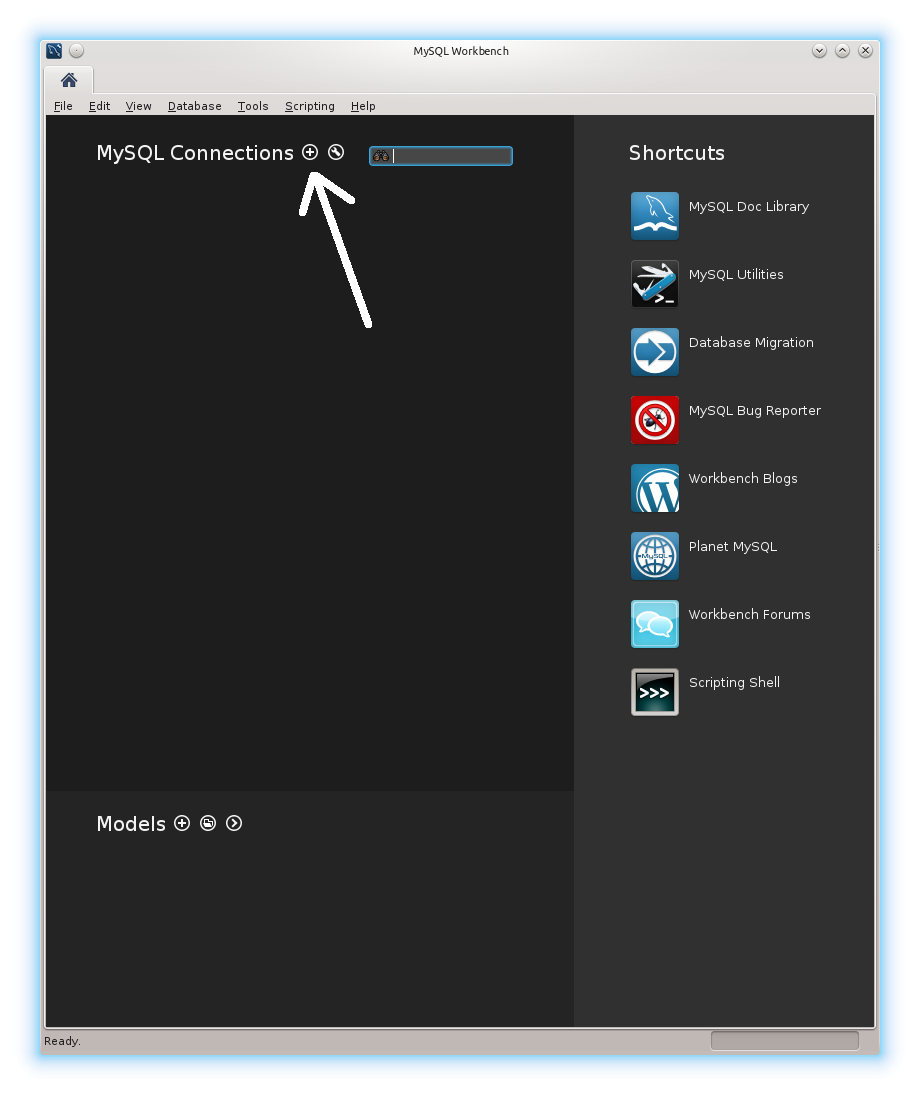
\includegraphics[width=\linewidth]{myndir/workbench-upphafsskjar-or}
\end{figure*}

\begin{figure*}
\caption[Tengingarskjár MySQL Workbench]{Tengingarskjár MySQL Workbench. Hér er verið að búa til tenginguna ``Prufutenging'', sem tengist MySQL-þjóni sem keyrir á sömu tölvu og Workbench-inn (127.0.0.1) með notandanafninu ``root''.}
\label{mynd:workbench-login}
\centering
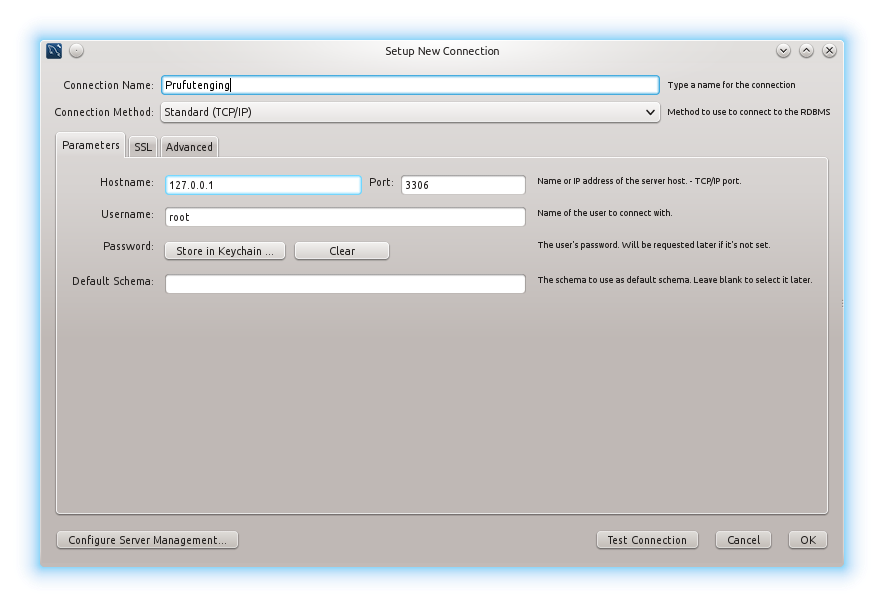
\includegraphics[width=\linewidth]{myndir/workbench-login}
\end{figure*}

\begin{figure*}
\caption[Nýr gagnagrunnur]{Nýr gagnagrunnur búinn til með MySQL Workbench. Efri örin vísar á hnappinn sem ýta þarf á til að keyra SQL-skipunina. Neðri örin vísar á lista af gagnagrunnum sem sýnilegir eru á servernum. Birtist gagnagrunnurinn sem búinn er til ekki um leið og skipunin er keyrð, hægri-smellið þá á listann og ``refresh''ið hann.}
\label{mynd:workbench-create-db}
\centering
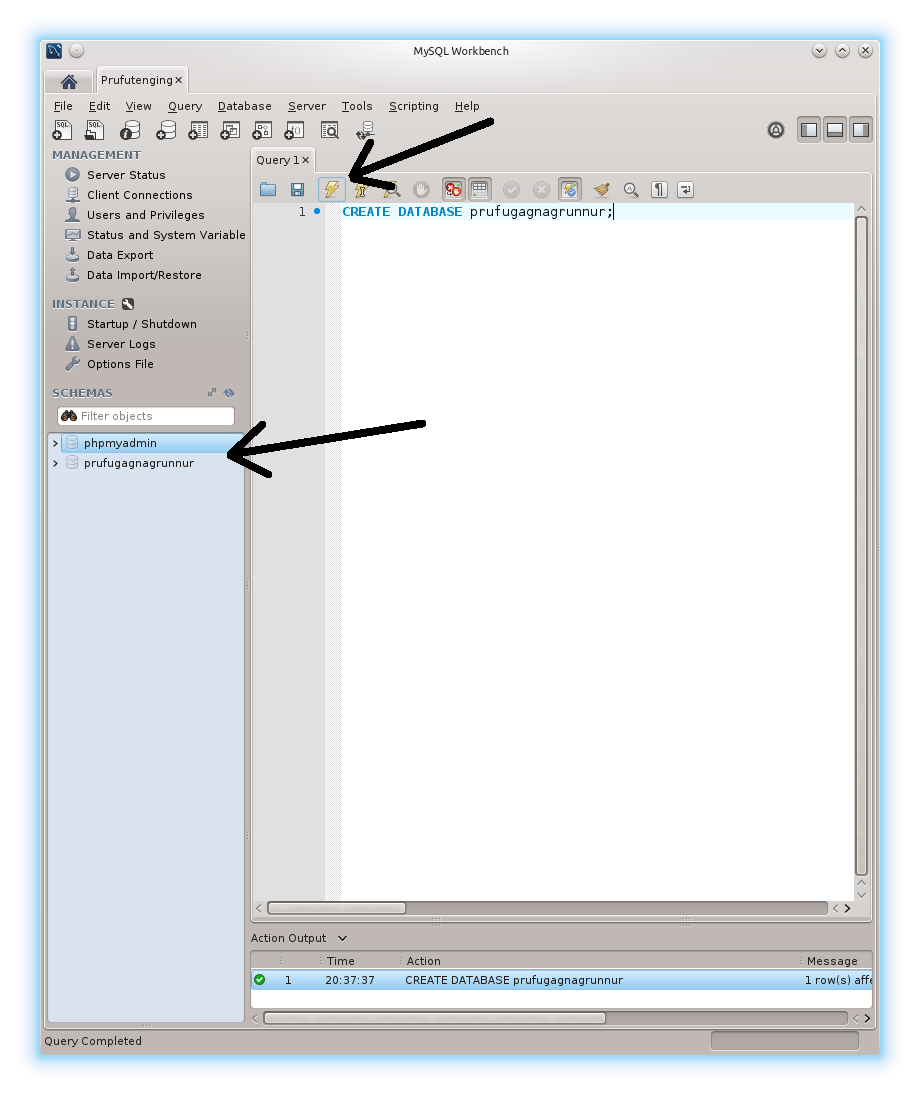
\includegraphics[width=0.8\linewidth]{myndir/workbench-create-db-or}
\end{figure*}

\begin{figure*}
\caption[Ný tafla]{Ný tafla búin til með MySQL Workbench. Skipunin er slegin inn í aðalgluggann og keyrð með ``eldingarhnappnum'' eins og skipunin á mynd \ref{mynd:workbench-create-db}.}
\label{mynd:workbench-create-table}
\centering
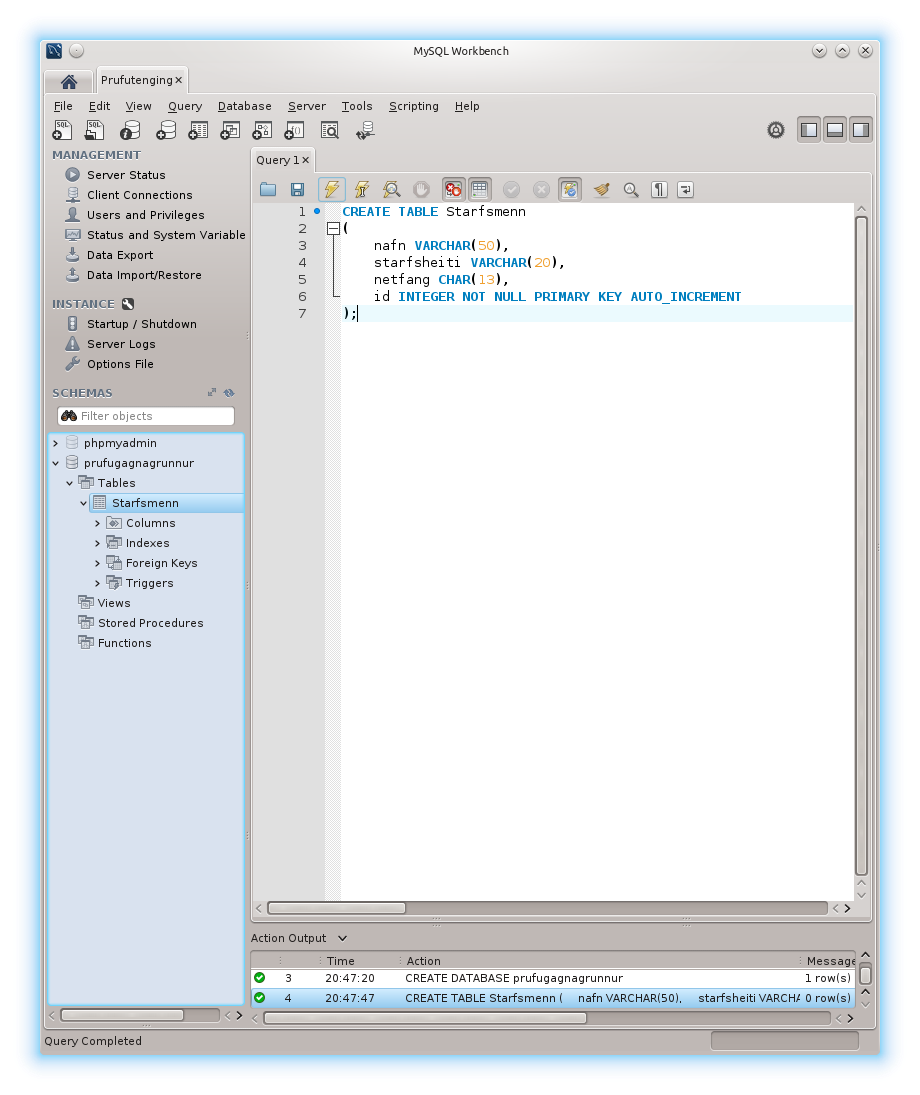
\includegraphics[width=0.8\linewidth]{myndir/workbench-create-table}
\end{figure*}

\section{Yfirlit}
Í þessum kafla fengum við örstutta kynningu því hvernig SQL-gagnagrunnar eru uppbyggðir og hvernig við getum átt við þá samskipti. 

Helstu atriðin eru:
\begin{itemize}
 \item Gögn í SQL-gagnagrunni má líta á sem raðir í töflum.
 \item SQL-skipanir eru notaðir til að skilgreina töflur og setja í þær gögn.
 \item Fyrirspurnir eru notaðar til að sækja gögn úr gagnagrunnum. Fyrirspurnir eru sérstök gerð SQL-skipana.
 \item SQL-skipanir má keyra úr aðalglugga MySQL Workbench.
\end{itemize}
Athuga ber að við höfum ekki farið yfir uppbyggingu skipananna. Það að læra á skipanirnar sjálfar er viðfangsefni næstu kafla.

\chapter{Uppsetning taflna}
\label{kafli:uppsetningtaflna}
Í kafla \ref{undirkafli:synidaemi-i-sql} sáum við dæmi um hvernig búa má til töflu með SQL-skipun. Hins vegar eyddum við ekki sérstaklega miklum tíma í að reyna að skilja hvernig skipunin er uppbyggð, hvað öll lykilorðin sem fram komu þýddu eða hvað er leyfilegt. Viðfangsefni kaflans sem við erum stödd í núna verður að leiðrétta þennan trassaskap og sökkva okkur í töflugerð.
\section{Að búa til töflu} % CREATE
Tökum skref aftur á bak frá og athugum hversu einfalda töflu við getum búið til. Hún er líklega eitthvað á þá leið sem sjá má á sýnidæmi \ref{sql:k3d1-create-table-fallegt}.

\begin{example}
\caption[Mjög einföld tafla]{Mjög einföld tafla. Athugum að ``NafnToflu'' og ``nafnDalks'' er ekki hluti af SQL-málinu, heldur bara dæmi um hvernig heiti á töflum og dálkum eru skilgreind.}
\label{sql:k3d1-create-table-fallegt}
\centering
\sql{sql/k3d1-create-table-fallegt.sql}
\end{example}

Skoðum þessa skipun nú mjög vandlega.
\begin{itemize}
 \item Hún hefst á að lýsa yfir hvað gera skal - hér er það \verb|CREATE TABLE|. Næst kemur nafn töflunnar fram.
 \item Þegar nafn töflunnar hefur verið gefið opnast svigi.
 \item Inni í sviganum kemur nafnið á einum dálki og orðið \verb|INTEGER|\footnote{Merkingin á þessum lykilorðum sem við höfum séð á eftir dálkheitunum, \emph{INTEGER} og \emph{VARCHAR}, útskýrist í næsta undirkafla (\ref{undirkafli:gagnagerdir}).}. Hér er einungis einn dálkur.
 \item Skipuninni lýkur á því að sviganum er lokað og semíkomma (;) sett á eftir.
\end{itemize}

Skoðum næst sýnidæmi \ref{sql:k3d2-create-table-meira-fallegt}, sem er \emph{örlítið} stærra.
\begin{example}
\caption{Einföld tafla}
\label{sql:k3d2-create-table-meira-fallegt}
\centering
\sql{sql/k3d2-create-table-meira-fallegt.sql}
\end{example}

Hér sjáum við ágætlega hvernig bæta má við öðrum dálki. Fyrsta dálklýsingin er skrifuð, síðan kemur komma, síðan fylgir næsta dálklýsing.

Athugum að engin komma er á eftir síðustu dálklýsingunni. Það er vegna þess að dálkarnir eru einungis \emph{aðskildir} með kommum, komman er ekki hluti af dálklýsingunni sjálfri.
\section{Innsetning gagna} % INSERT
\label{undirkafli:innsetning}
Þegar töflur eru búnar til með \verb|CREATE TABLE| skipun eru þær tómar. Til að fylla töflu með gögnum þarf að nota aðra skipun - \verb|INSERT|. Til að setja töluna $1$ inn í töfluna sem við bjuggum til með sýnidæmi \ref{sql:k3d1-create-table-fallegt} mætti nota \verb|INSERT| skipunina í sýnidæmi \ref{sql:k3d8-insert-einfalt}.

\begin{example}
\caption[INSERT í einfalda töflu]{INSERT í einfalda töflu. Þessi skipun setur töluna $1$ inn dálkinn \emph{nafnDalks}. Niðurstaðan er tafla \ref{tafla:insert-einfalt}.}
\label{sql:k3d8-insert-einfalt}
\centering
\sql{sql/k3d8-insert-einfalt.sql}
\end{example}

Skoðum þessa skipun í smáatriðum líka. 

\begin{itemize}
 \item Aftur hefst skipunin á því að lýsa því yfir hvað gera skal. Hér ætlum við að setja inn gögn - \verb|INSERT|. Við ætlum að setja gögnin inn í eitthvað, svo við segjum \verb|INSERT INTO|.
 \item Næst kemur nafn töflunnar sem gögnin eiga að fara í. %Gagnagrunnskerfið getur ekki giskað á hvert gögnin eiga að fara. %Við verðum að taka það fram.
 \item Svigi opnast, nafn dálksins sem gögnin eiga að fara inn í er skrifað og sviginn lokast.\footnote{Strangt til tekið er hægt að sleppa þessum sviga. Gagnagrunnskerfið reynir þá að setja gögnin inn í þá dálka sem það finnur í töflunni. Þessar ágiskanir geta verið til vandræða, betra er að venja sig á að taka dálkheitin alltaf fram.}
 \item Að lokum segjum við hvað við ætlum að setja inn. Það eru gögn (eða ``gildi'', \verb|VALUES|). Gögnin sem við ætlum að setja inn er ein lína, sem við afmörkum með svigum. Línan samanstendur af einni tölu. Sem fyrr lokum við skipuninni með semíkommu.
\end{itemize}

\begin{table}
\centering
\caption[Eftir einfalt INSERT]{Niðurstaðan eftir að sýnidæmi \ref{sql:k3d1-create-table-fallegt} og \ref{sql:k3d8-insert-einfalt} hafa verið keyrð - ofurlítil tafla með einum dálki og einni línu af gögnum.}
\label{tafla:insert-einfalt}
\begin{tabular}{l}
\toprule
nafnDalks\\
\midrule
1\\
\bottomrule
\end{tabular}
\end{table}

Mikilvægt er að vita að \verb|INSERT| skipun setur alltaf inn \emph{heila línu} af gögnum í töfluna. Sé taflan með fleiri en einn dálk (Flestar töflur sem ekki eru gagnslausar hafa fleiri en einn dálk.) þarf að skilgreina öll gögnin í einu. Sýnidæmi \ref{sql:k3d9-insert-margir-dalkar} er dæmi um slíkt.

\begin{example}
\caption[INSERT í tvo dálka í einu]{INSERT í tvo dálka í einu. Þessi skipun setur tölurnar $1$ og $2$ inn í sömu línu. Niðurstaðan er tafla \ref{tafla:insert-margir-dalkar}.}
\label{sql:k3d9-insert-margir-dalkar}
\centering
\sql{sql/k3d9-insert-margir-dalkar.sql}
\end{example}

\begin{table}
\centering
\caption[Eftir INSERT á línu]{Niðurstaðan eftir að sýnidæmi \ref{sql:k3d2-create-table-meira-fallegt} og \ref{sql:k3d9-insert-margir-dalkar} hafa verið keyrð. Tafla með tveimur dálkum og einni línu af gögnum.}
\label{tafla:insert-margir-dalkar}
\begin{tabular}{ll}
\toprule
nafnFyrstaDalks&nafnAnnarsDalks\\
\midrule
1&2\\
\bottomrule
\end{tabular}
\end{table}
Til að skrifa meira en eina línu af gögnum inn í gagnagrunn má keyra \verb|INSERT| skipun oftar en einu sinni. Væri skipunin í sýnidæmi \ref{tafla:insert-margir-dalkar} keyrð tvisvar myndi línan sem hún lýsir vera tvítekin í töflunni.

Það að skrifa alla \verb|INSERT INTO| romsuna upp upp á nýtt fyrir hverja línu sem setja skal inn getur verið þreytandi. Þess vegna býður MySQL upp á leið til að setja inn margar línur í einu. Við sjáum dæmi um það í sýnidæmi \ref{sql:k3d10-insert-margar-linur}.

\begin{example}
\caption[INSERT í tvo dálka í einu]{INSERT í tvo dálka í einu. Þessi skipun setur tölurnar $1$ og $2$ inn í eina línu og tölurnar $3$ og $4$ í þá næstu. Niðurstaðan er tafla \ref{tafla:insert-margar-linur}.}
\label{sql:k3d10-insert-margar-linur}
\centering
\sql{sql/k3d10-insert-margar-linur.sql}
\end{example}

\begin{table}
\centering
\caption[Eftir INSERT á tveimur línum]{Niðurstaðan eftir að sýnidæmi \ref{sql:k3d2-create-table-meira-fallegt} og \ref{sql:k3d10-insert-margar-linur} hafa verið keyrð. Tafla með tveimur dálkum og tveimur línum af gögnum.}
\label{tafla:insert-margar-linur}
\begin{tabular}{ll}
\toprule
nafnFyrstaDalks&nafnAnnarsDalks\\
\midrule
1&2\\
3&4\\
\bottomrule
\end{tabular}
\end{table}

\section{Algengar gagnagerðir: Tölur og texti} % INTEGER (INT), VARCHAR, CHAR
\label{undirkafli:gagnagerdir}
Einni stórri spurningu um \verb|CREATE TABLE| dæmin framar í þessum kafla er enn ósvarað - hvað er þetta \verb|INTEGER|?

Integer er dæmi um svokallaða gagnagerð\footnote{e. \emph{data type}}. Nánar til tekið er þetta gagnagerð sem táknar heiltölur, tölur eins og töluna $1$, töluna $-256$ og allar tölur sem við höfum sett inn í töflur framar í bókinni. Þegar \verb|INTEGER| kemur fyrir í dálkskilgreiningu erum við sem sagt að segja gagnagrunnskerfinu að við munum einungis geyma heiltölur í þessum dálki.

Skoðum nokkrar helstu gagnagerðir í MySQL og hvenær við notum þær.
\subsection{Heiltölur - INTEGER}
Fram hefur komið að \verb|INTEGER| dálkur geymi heiltölur. Hann tekur ekki við kommutölum.\footnote{Í stað \emph{INTEGER} má skrifa styttinguna \emph{INT}, sem hefur sömu áhrif.}

Lægsta talan sem slíkur dálkur getur geymt er $-2147483648$ og sú hæsta $2147483647$. Ástæðan fyrir því að lægri og hærri tölur en þessar valda villum er sú að MySQL notar einungis fjögur bæti til að geyma hverja heiltölu - hærri og lægri tölur komast ekki fyrir í svo litlu geymsluplássi.

Sé nauðsynlegt að geyma tölur sem ekki passa inn á þetta bil má nota gagnagerðina \verb|BIGINT| í stað \verb|INTEGER|. Slíkur dálkur geymir einnig heiltölur, en hefur átta bæti til að geyma hverja tölu. \verb|BIGINT| dálkur getur því geymt mun stærri (eða ``lengri'') tölur.

Sé vitað að tölurnar sem fara inn í dálkinn séu allar mjög litlar um sig má nota gagnagerðirnar \verb|TINYINT|, \verb|SMALLINT| og \verb|MEDIUMINT| í MySQL. Þær taka hver um sig $1$, $2$ og $3$ bæti til að geyma hverja tölu. Sjaldnast er ástæða til að nota þessar gagnagerðir í dag. Tafla þyrfti að innihalda tugi milljóna raða\footnote{Reyndar eru í dag til gagnagrunnstöflur sem innihalda \emph{hundruðir milljarða} raða.} til að plásssparnaðurinn gæti skipt máli á nútíma tölvukerfum.

\begin{table}
\centering
\caption[Heiltöludálkar]{Heiltölugagnagerðir í MySQL og stærðir þeirra.}
\label{tafla:heiltolur}
\begin{tabular}{llll}
\toprule
Nafn&Stærð í&Lægsta gildi&Hæsta gildi\\
&bætum&&\\
\midrule
\verb|TINYINT|&1&$-128$&$127$\\
\verb|SMALLINT|&2&$-32768$&$32767$\\
\verb|MEDIUMINT|&3&$-8388608$&$8388607$\\
\verb|INT|&4&$-2147483648$&$2147483647$\\
\verb|BIGINT|&8&$-9223372036854775808$&$9223372036854775807$\\
\bottomrule
\end{tabular}
\end{table}

Ef sérstök skilyrði koma ekki upp er best og einfaldast að halda sig við \verb|INTEGER| til að geyma heiltölur. Þetta getur sérstaklega borgað sig ef seinna reynist nauðsynlegt að færa gagnagrunninn á milli gagnagrunnskerfa - sum gagnagrunnskerfi styðja ekki allar gagnagerðirnar sem MySQL býður upp á. Gamla góða \verb|INTEGER| er hins vegar alltaf til staðar.

\newthought{Íslenskar kennitölur} eru varhugaverðar. Freistandi getur verið að geyma kennitölur í heiltöludálkum. Þær eru jú kommulausar tölur, ekki satt? Nokkur atriði leiða þó til þess að þær passa ekki mjög vel í slíka dálka.

\begin{itemize}
 \item Stærsta tala sem hægt er að geyma í venjulegum \verb|INTEGER| dálki er $2147483647$. Það þýðir að kennitölur allra sem fæddir eru á 22. degi mánaðar eða seinna komast ekki fyrir í dálkinum! \verb|BIGINT| þyrfti að nota.
 \item Kennitölur eru ekki notaðar eins og flestar tölur. Þær eru t.d. ekki lagðar saman eða bornar saman með $<$ og $>$ virkjum. Við þurfum oftar að skoða ákveðna stafi í kennitölunni (t.d. fimmta og sjötta stafinn til að komast að fæðingarári) frekar en stærð tölunnar sjálfrar.
 \item Kennitölur eru venjulega skrifaðar með bandstrikum, sem eiga ekki heima í heiltöludálki.
\end{itemize}
Vænlegra er að nota \verb|CHAR| dálk til að geyma kennitölur. Lítum á þá gagnagerð í næsta kafla!

\subsection{Texti - VARCHAR og CHAR}
Í forritun lítum við oftast á texta sem safn af stöfum, SQL er hér engin undantekning. Slíkt safn er kallað strengur\footnote{e. \emph{string}}. \verb|'Ari'|, \verb|'Ari sá sól'| og \verb|'Ari á 10 krónur'| eru allt dæmi um strengi. 

Eins og sjá má eru strengir afmarkaðir með gæsalöppum. Mikilvægt er að gleyma þeim ekki þegar strengir eru slegnir inn (sjá kafla \ref{undirkafli:innsetning}). Þær eru aðalleiðin sem gagnagrunnskerfið hefur til að vita hvort að um streng eða dálkheiti sé að ræða. 

Venja er að nota einfaldar gæsalappir (\verb|'|) í SQL til að afmarka strengi. Tvöfaldar gæsalappir (\verb|"|) virka líka í MySQL.

Talað er um að strengur hafi ákveðna \emph{lengd}. Lengd strengs er fjöldi stafa í strengnum, að bilum meðtöldum. Gæsalappirnar eru ekki taldar með, þær umlykja strenginn en eru ekki hluti af honum. Þannig er \verb|'Ari'| strengur af lengd 3, \verb|'Ari sá sól'| er strengur af lengd 10.

Strengir geta innihaldið næstum hvaða stafi sem er, líka tölustafi. \verb|'Ari á 10 krónur'| er löglegur strengur. Strengur getur meira að segja innihaldið ekkert nema tölustafi. \verb|"10"| er strengur, $10$ er heiltala.

\newthought{Til að geyma texta} höfum við nokkrar gagnagerðir, líkt og við höfum nokkrar gagnagerðir til að geyma heiltölur. Þær helstu eru \verb|CHAR| og \verb|VARCHAR|. ``Char'' stendur hér fyrir enska orðið ``character'', sem þýða má sem ``stafur''. ``Var'' í \verb|VARCHAR| stendur fyrir ``variable''. 

Þegar \verb|CHAR| og \verb|VARCHAR| gagnagerðirnar eru notaðar þurfum við að taka fram hversu langa strengi dálkurinn á að geta tekið við\footnote{Oft er talað um ``breidd'' á þessum dálkum. Til að strengur af lengd $5$ komist inn í dálk þarf dálkurinn að vera $5$ stafa breiður.}. Þetta er gert með því að setja hámarkslengdina inn í sviga. \verb|CHAR(3)| er dálkur sem tekur við strengjum af lengd 3.

Sé strengur sem er of langur settur inn í \verb|CHAR| eða \verb|VARCHAR| dálk er klippt af hægri enda hans svo að hann passi. Væri t.d. reynt að geyma \verb|'Ari sá sól'| í \verb|CHAR(5)| dálk væri útkoman \verb|'Ari s'|. 

Munurinn á \verb|CHAR| og \verb|VARCHAR| kemur fyrst og fremst fram þegar of \emph{stuttir} strengir eru settir inn í dálkinn. 
\begin{itemize}
 \item Sé strengur styttri en breidd \verb|CHAR| dálks sem hann er settur inn í er bilum bætt við hægri enda strengsins svo hann passi nákvæmlega. Þannig yrði strengurinn \verb|'Ari sá sól'| að \verb|'Ari sá sól     '| væri hann settur inn í \verb|CHAR(15)| dálk.
 \item Sé strengur sem er of stuttur settur inn í \verb|VARCHAR| dálk er hann einfaldlega geymdur eins og hann er. \verb|VARCHAR| dálkur getur geymt ``of stutta'' strengi.
\end{itemize}
\verb|CHAR| dálkur getur verið að hámarki 255 stafir að breidd. \verb|VARCHAR| dálkur getur verið allt að 65.535 stafa breiður.

Hljómi \verb|VARCHAR| hér eins og almennt gagnlegri gagnagerð er það líklega vegna þess að það er rétt. \verb|VARCHAR| eyðir minna plássi og breytir strengjum ekki að óþörfu. \verb|CHAR| dálkar eru gagnlegir þegar vitað er fyrirfram að allir strengir sem eiga að fara inn í dálkinn séu af sömu lengd eða ef seinni tíma vinnsla krefst þess að gögnin séu sjálum sér mjög samkvæm. Leiki vafi á er einfaldast að nota bara \verb|VARCHAR|.
\begin{marginfigure}
\caption[CHAR og VARCHAR]{Hvernig CHAR og VARCHAR dálkar geyma texta. Talan til vinstri táknar lengd strengsins eins og hann er geymdur.}
\label{mynd:char-varchar}
\centering
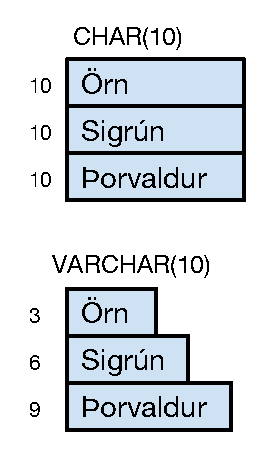
\includegraphics[width=\linewidth]{myndir/char-varchar}
\end{marginfigure}

\newthought{Mjög langur texti} getur verið erfiður í meðförum. Sé ætlunin t.d. að geyma bækur, bloggfærslur eða fréttagreinar í gagnagrunni, hversu stóran \verb|VARCHAR| dálk þyrfti til að halda utan um textann? Svarið er: Of stóran.

MySQL býður upp á aðrar gagnagerðir sem eru meira viðeigandi fyrir slíka vinnslu - hér eru helstar \verb|TEXT| og \verb|LONGTEXT|. \verb|LONGTEXT| dálkur er fær um að geyma strengi sem eru allt að 4 GiB að lengd.

Sé ætlunin að geyma upplýsingar sem almennt eru af skynsamlegri stærð, t.d. mannanöfn, þá er hagkvæmara að nota \verb|VARCHAR| dálk.

\section{Dæmi um töflur með tölum og texta}
Ýmsar töflur má búa til með tölum og texta. Fyrsta taflan sem við sáum, tafla \ref{tafla:starfsmenn-ts}, er dæmi um slíka töflu. Lítum á nokkur fleiri dæmi.
% TODO tengja þetta í texta


\begin{example}
\caption[Heiltölur]{CREATE TABLE skipun sem gæti búið til töflu \ref{tafla:heiltolur} í MySQL. Hér er einfaldur \emph{INTEGER} dálkur notaður til að geyma fjölda bæta, \emph{BIGINT} þarf til að geyma lengstu tölurnar.}
\label{sql:k3d3-heiltolur}
\centering
\sql{sql/k3d3-heiltolur.sql}
\end{example}

\begin{figure}
\caption[High Score tafla]{``High score'' tafla fyrir tölvuleik. Fyrir nokkrum áratugum litu high score listar í spilakössum yfirleitt út á þennan hátt. Hver lína samanstóð af þremur upphafsstöfum og stigafjölda. Hana mætti búa til með skipuninni í sýnidæmi \ref{sql:k3d4-high-score}.}
\label{mynd:high-score}
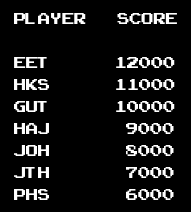
\includegraphics{myndir/high-score}
\end{figure}

\begin{example}
\caption[High Score tafla]{High score taflan á mynd \ref{mynd:high-score} búin til með SQL-skipun. Hér vitum við að spilararnir nota alltaf nákvæmlega þrjá upphafsstafi til að auðkenna sig, svo \emph{CHAR} dálkur er viðeigandi. Stigin sjálf eru geymd í \emph{INTEGER} dálki.}
\label{sql:k3d4-high-score}
\centering
\sql{sql/k3d4-high-score.sql}
\end{example}

\begin{figure}
\caption[Matseðill]{Hamborgaramatseðill á veitingastað. Töflur geta litið út á ýmsan hátt. Matseðil af þessari gerð mætti geyma í gagnagrunni, þó að hann líti e.t.v. ekki út eins og tafla við fyrstu sýn. Töflu sem heldur utan um upplýsingarnar á honum má sjá á sýnidæmi \ref{sql:k3d5-matsedill}. }
\label{mynd:matsedill}
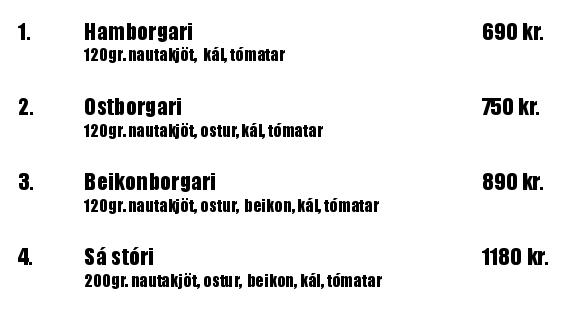
\includegraphics[width=\textwidth]{myndir/matsedill}
\end{figure}

\begin{example}
\caption[Matseðill]{SQL-framsetning á matseðlinum á mynd \ref{mynd:matsedill}. Við gerum ráð fyrir að lýsingin á réttinum þurfi meira pláss en nafn hans.}
\label{sql:k3d5-matsedill}
\centering
\sql{sql/k3d5-matsedill.sql}
\end{example}

\section{Fleiri gagnagerðir}
Þó að ýmislegt sé hægt að gera með einungis texta og heiltölum, þá býður MySQL upp á mun fleiri gagnagerðir. Lítum stuttlega á nokkrar.
\subsection{Tugabrot - DECIMAL}
Til að geyma tugabrot (kommutölur, t.d. $1,5$ og $5,2$) dugar \verb|INTEGER| dálkur ekki. Til þess getum við notað \verb|DECIMAL| dálk.

Til að búa til \verb|DECIMAL| dálk þurfum við að skilgreina tvær tölur. Sú fyrri er heildarfjöldi tölustafa sem mega vera í tölunni, sú seinni er fjöldi tölustafa ``hægra megin'' við kommuna. Þannig myndi \verb|DECIMAL(5,2)| dálkur passa akkúrat utan um töluna $123,45$.

\begin{table}
\centering
\caption[Eldsneyti]{Eldsneytisverð á bensínstöð. \emph{DECIMAL} dálkur er notaður til að halda utan um bensínverðið með nákvæmlega 1 aukastaf.}
\label{tafla:eldsneyti}
\begin{tabular}{lr}
\toprule
Gerð&Verð (kr.)\\
\midrule
95 oktan&$252,9$\\
Dísel&$242,3$\\
Vélaolía&$174,3$\\
98 oktan&$298,9$\\
\bottomrule
\end{tabular}
\end{table}

\begin{example}
\caption[Eldsneytisverð]{SQL-framsetning á eldsneytisverðinu í töflu \ref{tafla:eldsneyti}. Verðið er geymt í dálki sem tekur við tugabroti með fjóra markverða stafi, þar af einum fyrir aftan kommu. \emph{INSERT} skipun fylgir með (sjá nánar í kafla \ref{undirkafli:innsetning}). Athugum að \emph{INSERT} skipunin tekur við tölum á ensku formi, sem notar punkta þar sem kommur eru notaðar í íslensku (og öfugt). Væri reynt að setja tugabrotið inn með kommu væri það túlkað sem skipting á milli dálka!}
\label{sql:k3d6-eldsneyti}
\centering
\sql{sql/k3d6-eldsneyti.sql}
\end{example}

\subsection{Rauntölur - DOUBLE}
Það að þurfa að taka fram stærð talna getur verið mjög takmarkandi. Hvað ef skali talnanna er mjög mismunandi eða ef geyma þarf gríðarlega ``langar'' tölur? 

Massi sólarinnar er í kringum $1988550000000000000000000000000$ kg. Þessi tala passar ekki í nokkurn \verb|INTEGER| dálk - við þurfum að leita að öðrum lausnum.

\verb|DOUBLE| gagnagerðin getur geymt flestar tölur. Gallinn er sá að tölurnar í \verb|DOUBLE| dálki eru geymdar sem svokallaðar fleytitölur\footnote{e. \emph{floating point numbers}}, sem eru ekki fullkomlega nákvæmar. Þessi ónákvæmni er oftast afar smá, en getur verið til vandræða. Betra er að nota nákvæmar gagnagerðir (t.d. \verb|INTEGER| eða \verb|DECIMAL|) sé það mögulegt.

\begin{table}
\centering
\caption[Plánetur utan sólkerfisins.]{Nokkrar plánetur utan sólkerfisins sem líkjast jörðinni að einhverju leyti.}
\label{tafla:planetur}
\begin{tabular}{lll}
\toprule
Nafn&Fjarlægð (m)&Massi (kg)\\
\midrule
Gliese 667 Cc&$2,1475\cdot 10^{17}$&$2,6218\cdot10^{25}$\\
Kepler-62e   &$1,1353\cdot 10^{19}$&$2,1321\cdot10^{25}$\\
Tau Ceti e   &$1,1263\cdot 10^{17}$&$2,5680\cdot10^{25}$\\
Gliese 581 d &$1,9110\cdot 10^{17}$&$4,1686\cdot10^{25}$\\
\bottomrule
\end{tabular}
\end{table}

\begin{example}
\caption[Plánetur]{SQL-tafla sem haldið getur utan um pláneturnar í töflu \ref{tafla:planetur}. Fjarlægð þeirra frá okkar sólkerfi (í metrum) og massi þeirra (í kílóum) eru mjög óþjálar tölur, sem krefjast fleytitalna.}
\label{sql:k3d7-planetur}
\centering
\sql{sql/k3d7-planetur.sql}
\end{example}

\subsection{Dagsetningar - DATE}

\subsection{Rökbreytur - BOOLEAN}

\section{Tóm gildi} % NULL, NOT NULL
\section{Aðallyklar} %PRIMARY KEY
\section{Að eyða töflum} % DROP

\chapter{Fyrirspurnir}
\label{kafli:select}
Upplýsingar eru sjaldnast geymdar í gagnagrunnum gagnagrunnsins vegna. Markmiðið með að geyma upplýsingar er að gera það mögulegt að ná í þær aftur seinna.

Til að ná í upplýsingar notum við svokallaða \verb|SELECT| skipun. Þetta er skipun sem við munum koma til með að nota mikið og kynnast vel.

Hver \verb|SELECT| skipun er \emph{lýsing} á einhverjum upplýsingum sem við viljum fá. Við lýsum því hvaða upplýsingar við viljum, gagnagrunnskerfið sér svo um að finna hentuga leið til að finna þær fyrir okkur.
\section{SELECT}
Allar \verb|SELECT| skipanir innihalda í það minnsta lýsingu á því hvaða upplýsingar þarf að ná í.

Dæmi um ofurlitla \verb|SELECT| skipun má sjá í sýnidæmi \ref{sql:k4d1-summa}.

\begin{example}
\caption[Lágmarks SELECT]{Lítil \emph{SELECT} skipun. Hún inniheldur lýsingu á því hvaða upplýsingar á að finna: summuna $2+2$. Gagnagrunnskerfið getur reiknað hana út fyrir okkur.}
\label{sql:k4d1-summa}
\centering
\sql{sql/k4d1-summa.sql}
\end{example}

\subsection{SELECT - FROM}
Þegar \verb|SELECT| skipun er skrifuð er það oftast í þeim tilgangi að ná upplýsingum úr SQL-töflu.

Til þess að ná upplýsingum úr töflu með þarf að minnsta kosti að koma fram úr hvaða töflu og úr hvaða dálki upplýsingarnar eiga að koma. Þetta er gert með því að 

\begin{enumerate}
 \item Skrifa orðið \verb|SELECT| (sem gerir skipunina að \verb|SELECT| skipun)
 \item Skrifa nöfn dálkanna sem velja skal
 \item Skrifa orðið \verb|FROM|
 \item Skrifa nafn töflunnar sem velja skal úr.
\end{enumerate}

Dæmi um þetta má sjá á sýnidæmi \ref{sql:k4d2-from}.

\begin{table}
\centering
\caption[Nemendur]{Nokkrir uppskáldaðir nemendur fæddir árið 1998.}
\label{tafla:nemendur}
\begin{tabular}{llll}
\toprule
numer&nafn&kennitala&innritun\\
\midrule
1&Magnús Ásgeir Steinþórsson&090698-6489& 2014-07-01\\
2&Sigurður Ómarsson&251198-1369& 2014-06-04\\
3&Róbert Marinó Björnsson&060998-2489& 2014-07-14\\
4&Konráð Hreinn Aðalsteinsson&120498-8869& 2014-06-02\\
5&Jón Guðmundsson&230598-2159& 2014-07-03\\
6&Birgir Torfason&170798-7249& 2014-06-06\\
7&Höskuldur Frímann Ásmundsson&020298-4139& 2014-07-08\\
8&Jón Guðmundsson&210498-7889& 2014-06-11\\
9&Hilmar Hjartarson&020798-4599& 2014-07-16\\
10&Reynir Rafn Sigurgeirsson&211298-7239& 2014-06-12\\
11&Ingunn Rún Andradóttir&161298-1589& 2014-07-05\\
12&Pálína Björk Þórólfsdóttir&030798-0829& 2014-06-09\\
13&Regína Sigrún Jensdóttir&140798-6499& 2014-07-08\\
14&Líney Geirsdóttir&111098-3289& 2014-06-21\\
15&Steinunn Berglind Eiðsdóttir&190398-1889& 2014-07-04\\
16&Kristjana Ólafsdóttir&230298-4759& 2014-06-01\\
17&Þóra Gestsdóttir&010498-8489& 2014-07-05\\
18&Kolfinna Svava Óttarsdóttir&210498-5759& 2014-06-02\\
19&Elísabet Hrannarsdóttir&050298-3109& 2014-07-09\\
20&Hafrún Þorláksdóttir&250498-2849& 2014-06-19\\
\bottomrule
\end{tabular}
\end{table}

\begin{example}
\caption[SELECT FROM]{\emph{SELECT} skipun með \emph{FROM} klausu. Hún velur allan ``nafn'' dálkinn úr töflunni Nemendur (\ref{tafla:nemendur}).}
\label{sql:k4d2-from}
\centering
\sql{sql/k4d2-from.sql}
\end{example}

\begin{figure*}
\caption[Niðurstöður SELECT í Workbench]{Hér sést hvernig keyra má \emph{SELECT} skipunina úr sýnidæmi \ref{sql:k4d2-from} í MySQL Workbench. Skipunin er í aðalglugganum, niðurstaða hennar sést fyrir neðan.}
\label{mynd:workbench-select}
\centering
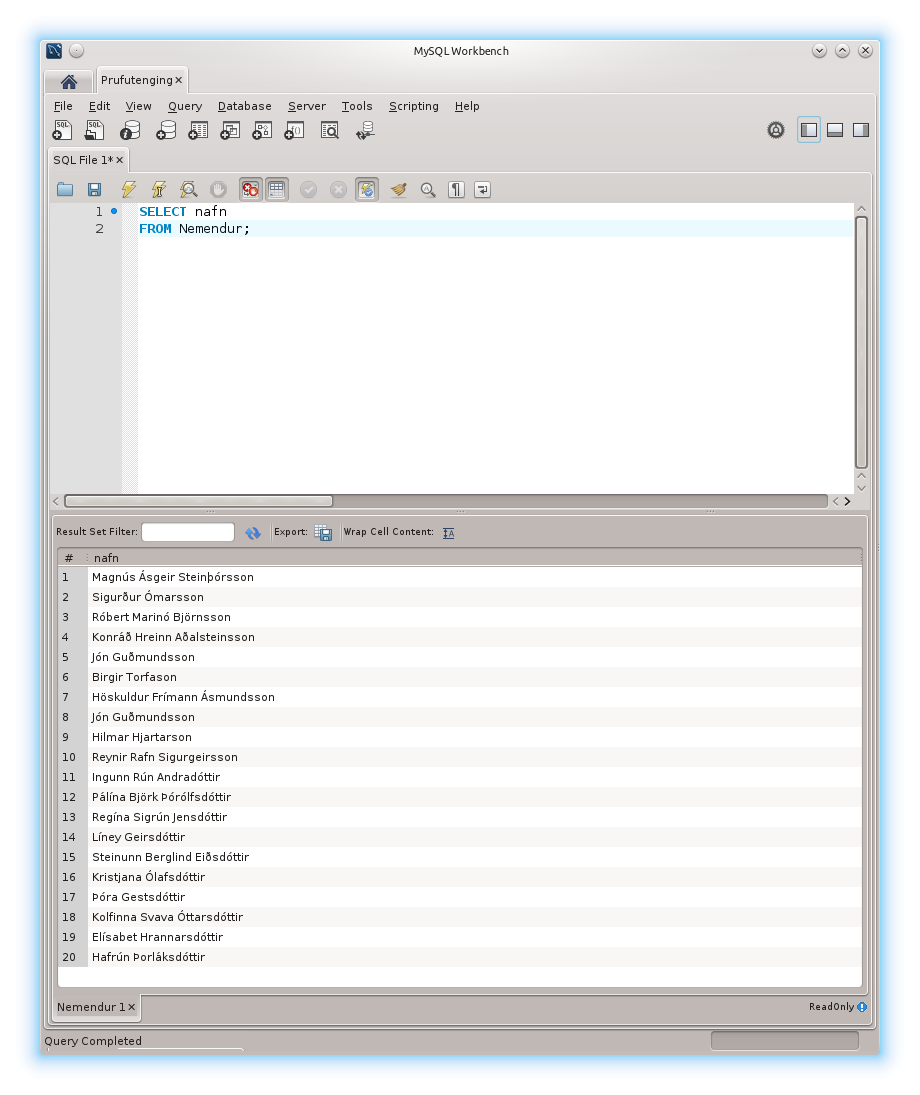
\includegraphics[width=\linewidth]{myndir/workbench-select}
\end{figure*}

\verb|SELECT| skipun getur náð í marga dálka (eða mörg atriði) í einu. Atriðin eru þá einfaldlega aðgreind með kommum. Þetta má sjá á sýnidæmi \ref{sql:k4d3-margir-dalkar}.

\begin{example}
\caption[SELECT með mörgum dálkum]{\emph{SELECT} skipun sem nær í marga dálka. }
\label{sql:k4d3-margir-dalkar}
\centering
\sql{sql/k4d3-margir-dalkar.sql}
\end{example}

\begin{table}
\centering
\caption[Niðurstaða margra dálka SELECT]{Niðurstaða skipunarinnar í sýnidæmi \ref{sql:k4d3-margir-dalkar} gæti litið út á þessa leið. Allar upplýsingarnar úr dálkunum ``nafn'' og ``kennitala'' voru valdar. Aðrir dálkar sjást ekki.}
\label{tafla:margir-dalkar-nidurstada}
\begin{tabular}{ll}
\toprule
nafn&kennitala\\
\midrule
Magnús Ásgeir Steinþórsson&090698-6489\\
Sigurður Ómarsson&251198-1369\\
Róbert Marinó Björnsson&060998-2489\\
Konráð Hreinn Aðalsteinsson&120498-8869\\
Kári Jensson&230598-2159\\
Birgir Torfason&170798-7249\\
Höskuldur Frímann Ásmundsson&020298-4139\\
Styrmir Hreinsson&210498-7889\\
Hilmar Hjartarson&020798-4599\\
Reynir Rafn Sigurgeirsson&211298-7239\\
Ingunn Rún Andradóttir&161298-1589\\
Pálína Björk Þórólfsdóttir&030798-0829\\
Regína Sigrún Jensdóttir&140798-6499\\
Líney Geirsdóttir&111098-3289\\
Steinunn Berglind Eiðsdóttir&190398-1889\\
Kristjana Ólafsdóttir&230298-4759\\
Þóra Gestsdóttir&010498-8489\\
Kolfinna Svava Óttarsdóttir&210498-5759\\
Elísabet Hrannarsdóttir&050298-3109\\
Hafrún Þorláksdóttir&250498-2849\\
\bottomrule
\end{tabular}
\end{table}

\begin{figure*}
\caption[Niðurstöður margra dálka SELECT í Workbench]{Hér sést hvernig sýnidæmi \ref{sql:k4d3-margir-dalkar} og niðurstaða \emph{SELECT} skipunarinnar sem í því er (tafla \ref{tafla:margir-dalkar-nidurstada}) getur litið út í MySQL Workbench.}
\label{mynd:workbench-nidurstada-margir-dalkar}
\centering
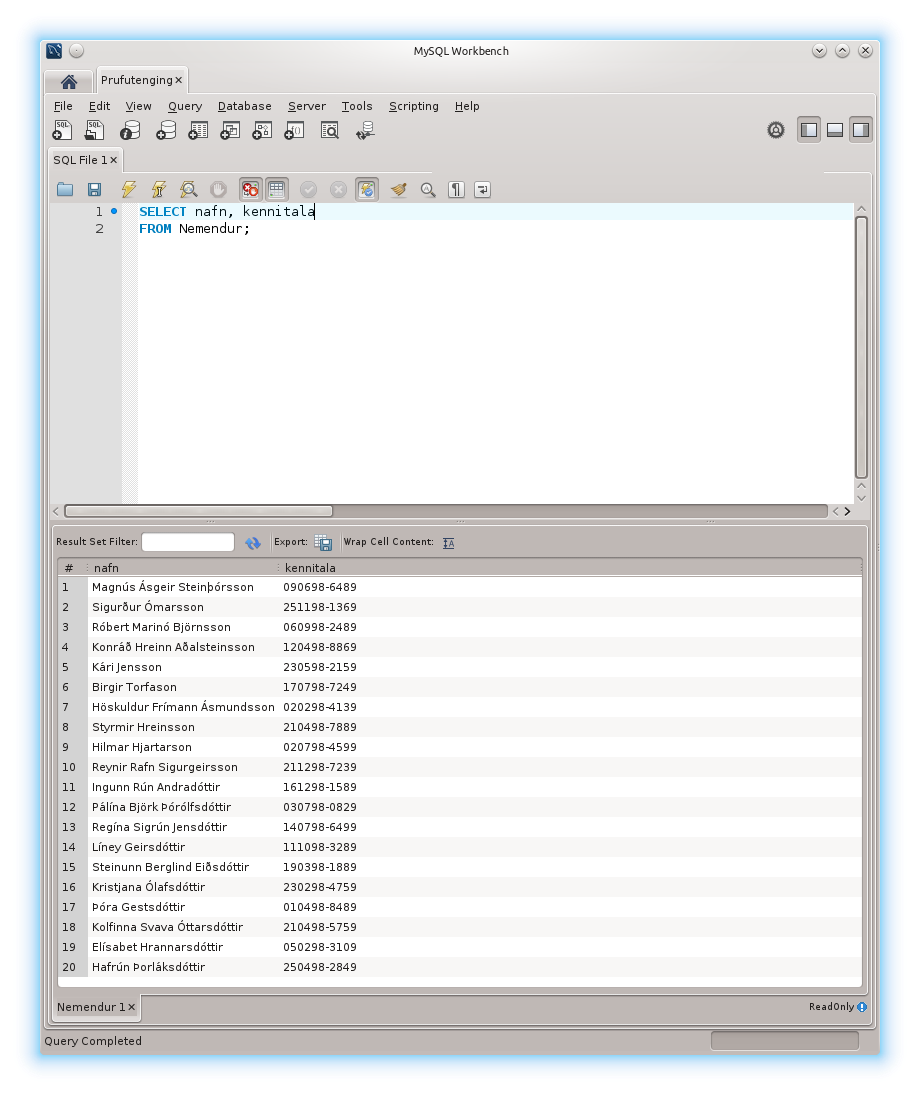
\includegraphics[width=\linewidth]{myndir/workbench-nidurstada-margir-dalkar}
\end{figure*}
\subsection{WHERE klausan}
Hingað til höfum við valið heila dálka með \verb|SELECT| skipunum. Það sem við viljum hins vegar oftast gera er að finna ákveðnar upplýsingar í töflunni, frekar en að fá þær allar.

Til þess að fá bara þær upplýsingar sem við viljum búum við til ``síu'' sem hleypir engum upplýsingum í gegn nema þeim sem við viljum.

Slík sía þarf að innihalda lýsingu á þeim gögnum sem hleypa á í gegn. Það er gert í klausu sem við köllum \verb|WHERE| klausu og kemur fyrir aftan \verb|FROM| klausuna. Dæmi um þetta má sjá í sýnidæmum \ref{sql:k4d4-where-numer} til \ref{mynd:workbench-nidurstada-jon}.

\begin{example}
\caption[SELECT með WHERE klausu - eftir númeri]{\emph{SELECT} skipun með \emph{WHERE} klausu sem nær í nafn nemanda (úr töflu \ref{tafla:nemendur}) þar sem ``numer'' dálkurinn er með gildið 11. Hún skilar einni línu, nafninu Ingunn Rún Andradóttir.}
\label{sql:k4d4-where-numer}
\centering
\sql{sql/k4d4-where-numer.sql}
\end{example}

\begin{example}
\caption[SELECT með WHERE klausu - eftir nafni]{\emph{SELECT} skipun með \emph{WHERE} klausu sem nær í kennitölu nemanda eftir nafni hans. Hún skilar einni línu, kennitölunni 251198-1369.}
\label{sql:k4d5-where-nafn}
\centering
\sql{sql/k4d5-where-nafn.sql}
\end{example}

\begin{example}
\caption[SELECT með WHERE klausu - endurtekin gildi]{Skilyrðið sem sett er fram í \emph{WHERE} klausu getur átt við meira en eina línu í töflunni. Þessi skipun finnur nöfn og kennitölu allra sem heita Jón Guðmundsson. Þeir reynast vera tveir, með kennitölurnar 230598-2159 og 210498-7889.}
\label{sql:k4d6-where-nafn-endurtekid}
\centering
\sql{sql/k4d6-where-nafn-endurtekid.sql}
\end{example}

\begin{figure*}[h]
\caption[Niðurstöður margra dálka SELECT í Workbench]{Hér sést sýnidæmi \ref{sql:k4d6-where-nafn-endurtekid} í MySQL Workbench.}
\label{mynd:workbench-nidurstada-jon}
\centering
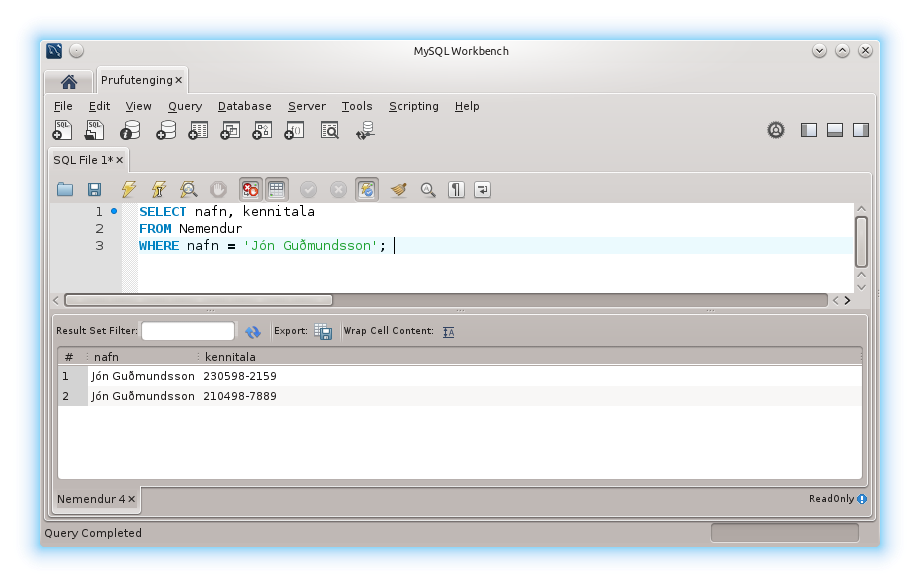
\includegraphics[width=\linewidth]{myndir/workbench-nidurstada-jon}
\end{figure*}
\subsection{Samanburðir í WHERE}
Í öllum \verb|WHERE| klausunum hér á undan er um að ræða síur sem henda öllu sem ekki uppfylla eitt, nákvæmt skilyrði. Skilyrðið í sýnidæmi \ref{sql:k4d4-where-numer}, \verb|numer = 11|, hleypir til dæmis einungis þeim nemanda sem er með nákvæmlega númerið 11 í gegn.

Skilyrðin geta þó verið margs konar. Skilyrðið \verb|numer > 11| hleypir til dæmis öllum línum í gegn þar sem gildið í ``numer'' dálkinum er stærra en 11. Yfirlit yfir mögulega samanburði má sjá á töflu \ref{tafla:samanburdir}.

\begin{table*}
\centering
\caption[Samanburðir]{Samanburðir sem nota mætti í \emph{WHERE} klausu \emph{SELECT} skipunar. Hér er \emph{numer} nafnið á dálki sem inniheldur tölur.}
\label{tafla:samanburdir}
\begin{tabular}{ll}
\toprule
Dæmi&Útskýring\\
\midrule
\emph{numer} = 5&Hleypir þeim línum í gegn þar sem gildið í \emph{numer} er nákvæmlega 5.\\
\emph{numer} > 5&Hleypir þeim línum í gegn þar sem gildið í \emph{numer} er stærra en 5.\\
\emph{numer} < 5&Hleypir þeim línum í gegn þar sem gildið í \emph{numer} er minna en 5.\\
\emph{numer} >= 5&Hleypir þeim línum í gegn þar sem gildið í \emph{numer} er 5 eða stærra.\\
\emph{numer} >= 5&Hleypir þeim línum í gegn þar sem gildið í \emph{numer} er 5 eða minna.\\
\emph{numer} != 5 eða \emph{numer} <> 5&Hleypir þeim línum í gegn þar sem gildið í \emph{numer} er ekki 5.\\
\bottomrule
\end{tabular}
\end{table*}
\section{LIKE og ``wildcards''}
\section{Mörg aðskilin skilyrði} % AND, OR, IN
\section{Helstu einindaföll}
\subsection{LENGTH}
\subsection{ROUND}
\subsection{UCASE og LCASE}
\section{GROUP BY}
\section{Helstu samsteypuföll}
\subsection{SUM og AVG}
\subsection{MIN og MAX}
\subsection{COUNT}
\section{HAVING}
\section{ORDER BY}
\subsection{LIMIT}
\section{Yfirlit}
\subsection{Uppbygging SELECT skipunarinnar}

\chapter{Að setja upp gagnagrunn}
\label{kafli:uppsetninggagnagrunns}
Við höfum kynnst því hvernig búa má til töflur (kafli \ref{kafli:uppsetningtaflna}) og hvernig ná má í gögn úr töflunum (kafli \ref{kafli:select}). 

Þessi vitneskja getur komið okkur furðu langt - en ekki alveg nógu. Nú skulum við skoða hvernig vinna má með stærri töflur og margar töflur í sama grunninum.
\section{Lyklar}
\label{undirkafli:lyklar}
Lyklar\footnote{e. \emph{key} eða \emph{index}} eru mikilvægir í öllum skilvirkum gagnagrunnum. Lyklar eru m.a. notaðir til að gera fyrirspurnir hraðvirkari og til að tengja töflur saman.

Lyklar eru stundum kallaðir \emph{vísar}. ``Lykill'' og ``vísir'' þýða það sama þegar kemur að MySQL.
\subsection{Almennt um lykla - KEY/INDEX}
Ímyndum okkur að við séum að leita að bók sem geymd er á mjög frumstæðu bókasafni. Á þessu bókasafni eru nefnilega engir titlar á kili bókanna og allar bækurnar líta eins út.
Erfitt verk, ekki satt? Að meðaltali þyrftum við að fara í gegnum hálft bókasafnið áður en við rekumst á bókina sem við viljum.

Þetta er verkið sem stendur frammi fyrir gagnagrunnskerfum í hvert skipti sem við notum þau til að leita að gögnum í dálki sem ekki er með lykil.
Gagnagrunnskerfi geta ekki borið saman gögn án þess að lesa þau.
Sem betur fer eru tölvur mjög fljótar að bryðja sér leið í gegn um mikið magn af gögnum - en við getum gert betur en að geyma allar upplýsingarnar okkar ómerktar og óraðar.

Það að setja vísi á dálk í gagnagrunnstöflu samsvarar því að búa til bókasafnskerfi sem getur sagt okkur í hvaða hillum og hvar í hillunum við getum fundið hverja bók. Það gefur auga leið að þetta gerir leitina auðveldari.

Hver tafla getur haft marga lykla.
\subsection{Einkvæmir lyklar - UNIQUE KEY}
Hægt er að setja þá takmörkun á lykil að öll stök sem honum tilheyra þurfi að vera einstök.

Slíkur lykill, sem kalla má einkvæman lykil\footnote{e. \emph{unique key} eða \emph{unique index}}, hefur þá ekki einungis það hlutverk að gera leit í gagnagrunninum auðveldari, heldur einnig það hlutverk að passa upp á að gögnin séu einstök.

Íslenskar kennitölur eru dæmi um gögn sem oft væri gott að vera með einkvæman lykil á. Það að fletta upp kennitölum er algeng aðgerð og við vitum að allar kennitölur eiga að vera einstakar.
\subsection{Aðallyklar - PRIMARY KEY}
\label{undirkafli:adallyklar}
Við höfum kynnst aðallyklum áður. Við sáum útskýringu á hvernig búa má til slíkan lykil í undirkafla \ref{undirkafli:adallyklar-kynning}.

Nú getum við séð að aðallykill er ekkert annað en sérstök gerð af einkvæmum lykli. Aðallykill er lykill sem hefur það sérstaka hlutverk að einkenna hverja línu fyrir sig, svo að hægt sé að vísa í hana á ótvíræðan hátt.

Þar sem að aðallykill töflu á að geta einkennt hverja línu er oftast best að lykillinn sé ekki byggður á gögnunum í línunni \footnote{af því að við viljum alls ekki þurfa að breyta aðallykli línu ef að gögnin breytast}. Einnig er gott að aðallykillinn sé lítill og einfaldur\footnote{Vegna þess að hann er oftast mikið notaður af gagnagrunnskerfinu.}. 

Kennitölur eru þess vegna ekki sérstaklega góðir aðallyklar. Þær geyma upplýsingar um einstaklinginn (fæðingardagsetningu hans), þær geta breyst (þó það sé sjaldgæft) og þær eru langar (sem er tímafrekt að lesa). Þess vegna eru romsur á borð við þá sem við höfum séð í \verb|CREATE TABLE| skipunum, \verb|id INTEGER NOT NULL PRIMARY KEY AUTO_INCREMENT| mikið notaðar til að skilgreina aðallykla. Þær búa til lykla sem 
\begin{itemize}
 \item Auðkenna línuna fullkomlega
 \item Eru heiltölur (og þar með litlar og auðveldar í vinnslu)
 \item Eru aldrei \verb|NULL|
 \item Og eru óháðir gögnunum.
\end{itemize}
Þó að tafla geti verið með marga lykla, þá er hver tafla aðeins með einn aðallykil.

\begin{example}
\caption[PRIMARY KEY]{Til upprifjunar: aðallykill skilgreindur sem hluti af \emph{CREATE TABLE} skipun. Þessi skipun býr til töflu \ref{tafla:nemendur}, sem við notuðum mikið í síðasta kafla.}
\label{sql:k5d1-primary-key}
\centering
\sql{sql/k5d1-primary-key.sql}
\end{example}
\subsection{(Ekki) meira um lykla}
Lyklar eru stórt viðfangsefni sem ekki er hægt að snerta á nema að mjög litlu leyti í þessari bók. Við munum ekki kafa dýpra í þá hér, heldur munum við láta þá bíða bóka og námskeiða fyrir lengra komna.

Í bili, þá skulum við láta okkur duga að muna að
\begin{itemize}
 \item Lyklar eru mikilvægir til að gagnagrunnskerfi geti unnið á skilvirkan hátt
 \item Við kunnum að búa til aðallykla 
 \item Aðallyklar geta auðkennt hverja línu í gagnagrunninum fyrir sig.
\end{itemize}
Síðasta atriðið verður sérstaklega mikilvægt þegar við förum að nota margar töflur í sama gagnagrunninum.
\section{Margar töflur í sama gagnagrunninum}
Við komumst að því strax í kafla \ref{kafli:fyrstuskrefin} að gagnagrunnur getur innihaldið margar töflur. Hingað til höfum við samt verið að vinna með töflur eina í einu, óháð hvor annarri.

Lítum á dæmi um hvernig tvær töflur sem eru staddar í sama gagnagrunni geta tengst. Skoðum aftur áfangatöfluna okkar frá því í síðasta kafla (\ref{tafla:afangar-aftur}).

\begin{table}
\centering
\caption[Áfangar]{Tafla \ref{tafla:afangar} endurtekin.}
\label{tafla:afangar-aftur}
\begin{tabular}{llll}
\toprule
numer&audkenni&fag&onn\\
\midrule
1&	FOR1A3U&	Forritun&		1\\
2&	VSH1A3U&	Vefhönnun&		1\\
3&	GSÖ1G2U&	Notkun gagnasafna&	1\\
4&	TÆK1A1U&	Tölvutækni&		1\\
5&	FOR1B3U&	Forritun&		2\\
6&	VSH2A3U&	Vefhönnun&		2\\
7&	GSÖ1F2U&	Notkun gagnasafna&	2\\
8&	TÆK2A3U&	Tölvutækni&		2\\
9&	FOR2B2U&	Forritun&		3\\
10&	VSH2B2U&	Vefhönnun&		3\\
11&	GSÖ2B2U&	Notkun gagnasafna&	3\\
12&	TÆK2B2U&	Tölvutækni&		3\\
13&	GRU2L4U&	Lokaverkefni grunndeildar&3\\
\bottomrule
\end{tabular}
\end{table}

Sú tafla er ágæt, en við getum gert hana betri með því að skipta henni upp í tvær töflur sem eru tengdar saman.\footnote{Af hverju er betra að vera ekki með svona endurtekningar? Hér má til dæmis nefna minni plásseyðslu og hversu mikið auðveldara verður að uppfæra gildin í töflunum séu engar endurtekningar til staðar.} Tökum eftir því að nafnið á hverju fagi er endurtekið í dálkinum \emph{fag}. 

Við gætum komist hjá þessari endurtekningu með því að geyma nöfnin á fögunum í sérstakri töflu.\footnote{Það sem við erum að gera hér er kallað að ``normalísera'' (e. \emph{normalize}) gagnagrunninn. Normalísering er viðfangsefni fyrir lengra komna.} Sú tafla gæti verið eins og tafla \ref{tafla:fog}.
Þar má sjá að við höfum gefið hverju fagi númer. Gefum okkur það að dálkurinn sem inniheldur þau númer sé aðallykill (sjá undirkafla \ref{undirkafli:adallyklar}). Þá getum við notað númerin til þess að vísa í línurnar. Þetta hefur verið gert á töflu \ref{tafla:afangar-fagnumer}, nöfnunum á fögunum hefur verið skipt út fyrir númer þeirra í töflu \ref{tafla:fog}.

\begin{table}
\centering
\caption[Fög]{Fög, sem áður voru í gömlu áfangatöflunni (\ref{tafla:afangar}/\ref{tafla:afangar-aftur}). Þessa töflu má tengja við endurbættu áfangatöfluna - töflu \ref{tafla:afangar-fagnumer}.}
\label{tafla:fog}
\begin{tabular}{ll}
\toprule
numer&fag\\
\midrule
1&Forritun\\
2&Vefhönnun\\
3&Notkun gagnasafna\\
4&Tölvutækni\\
5&Lokaverkefni grunndeildar\\
\bottomrule
\end{tabular}
\end{table}

\begin{table}
\centering
\caption[Áfangar - endurbætt]{Áfangataflan, þar sem nöfnunum á fögunum hefur verið skipt út fyrir númer þeirra, sem birtast í töflu \ref{tafla:fog}.}
\label{tafla:afangar-fagnumer}
\begin{tabular}{llll}
\toprule
numer&audkenni&fagNumer&onn\\
\midrule
1&	FOR1A3U&	1&	1\\
2&	VSH1A3U&	2&	1\\
3&	GSÖ1G2U&	3&	1\\
4&	TÆK1A1U&	4&	1\\
5&	FOR1B3U&	1&	2\\
6&	VSH2A3U&	2&	2\\
7&	GSÖ1F2U&	3&	2\\
8&	TÆK2A3U&	4&	2\\
9&	FOR2B2U&	1&	3\\
10&	VSH2B2U&	2&	3\\
11&	GSÖ2B2U&	3&	3\\
12&	TÆK2B2U&	4&	3\\
13&	GRU2L4U&	5&	3\\
\bottomrule
\end{tabular}
\end{table}

Hægt er að búa til mjög stórar fjölskyldur af töflum með því að tengja þær saman á þennan hátt með sameiginlegum gildum.

\begin{figure}
\caption[Tengsl taflna]{Sýnir hvernig töflur \ref{tafla:fog} og \ref{tafla:afangar-fagnumer} tengjast saman á dálkunum \emph{fagNumer} og \emph{fag}. (Töflurnar eru ekki sýndar í heilu lagi.)}
\label{mynd:tengsl}
\centering
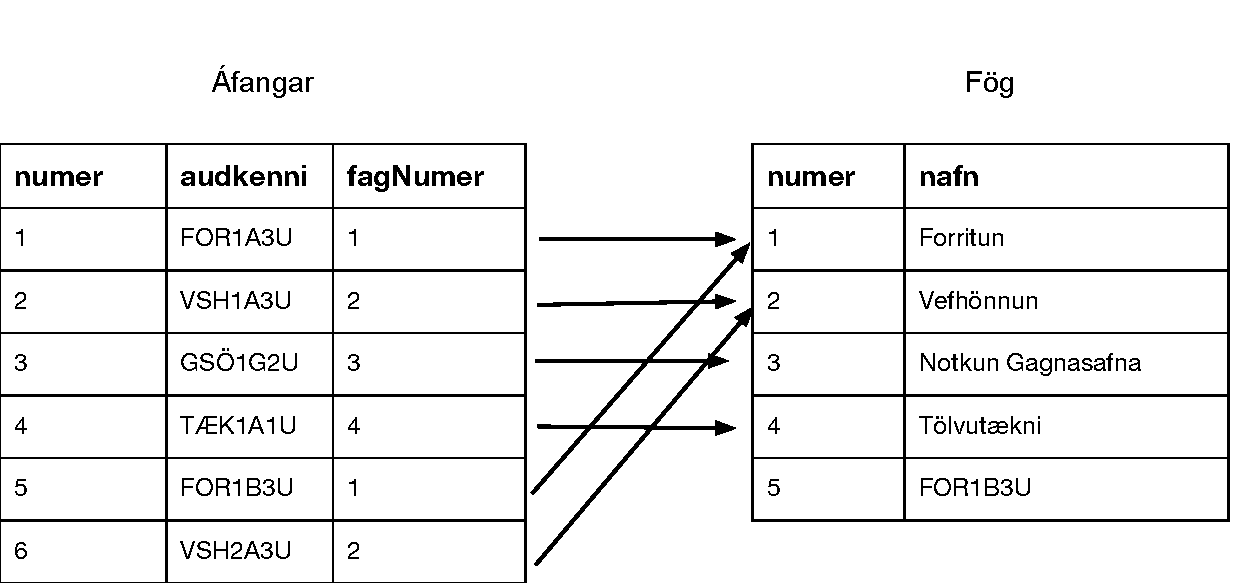
\includegraphics[width=\linewidth]{myndir/foreign-key}
\end{figure}

\section{Aðkomulyklar} % FOREIGN KEY
Þegar gildi í dálki eiga að vísa í línur annarrar töflu er hægt að tryggja sambandið með því að búa til svokallaðan aðkomulykil\footnote{e. \emph{Foreign key}.}.

Aðkomulykill myndar formlegt samband á milli tveggja taflna. Taflan sem inniheldur gögnin sjálf er kölluð foreldrið í sambandinu. Taflan sem inniheldur vísunina í gögnin er kölluð barnið\footnote{e. \emph{parent table} annars vegar og \emph{child table} hins vegar}. Í dæminu okkar á undan er \ref{tafla:fog} því foreldrið og \ref{tafla:afangar-fagnumer} barnið.

Aðkomulykillinn passar upp á að barnið geti ekki vísað í gögn sem ekki eru til í foreldrinu. Sé reynt að nota \verb|INSERT| skipun á barnið til að setja inn vísun í línu sem ekki er til í foreldrinu veldur það villu sé lykillinn rétt upp settur.

Aðkomulykillinn er skilgreindur í \verb|CREATE TABLE| skipun barnsins.

Mikilvægt er að dálkarnir í barninu og foreldrinu passi saman m.t.t. gagnagerðar (\ref{undirkafli:gagnagerdir}). Oftast er tengt saman á heiltöludálkum (sem þurfa að vera af sömu stærð).

Dálkurinn í foreldrinu sem aðkomulykillinn vísar í þarf að hafa aðallykill eða einkvæman lykill. Væri svo ekki gæti gagnagrunnskerfið ekki verið visst um hvaða línu í foreldrinu vísunin í barninu ætti við.
\section{Tengingar} % 1-1, 1-N, N-N









\chapter{Gagnavinnsla með mörgum töflum}
\label{kafli:gagnavinnslamargartoflur}
Við höfum komist að því hvernig búa má til töflur sem vísa hver í aðra. Við höfum líka komist að því hvernig ná má í upplýsingar úr einni töflu.

Nú skulum við líta á hvernig búa má til skipanir sem velja upplýsingar úr fleiri en einni töflu. Til þess þurfum við að læra hvernig stækka má \verb|FROM| klausuna svo að hún geti meðhöndlað margar töflur.
\section{Nöfn dálka}
Áður en lengra er haldið skulum við skoða betur dálitla ónákvæmni sem við höfum sætt okkur við hingað til.

Þegar við höfum vísað í dálk hefur okkur dugað að skrifa einfaldlega nafn hans. Við höfum ekki séð mikið að því að skrifa \verb|WHERE| klausur á borð við \verb|WHERE numer = 11|.

Þetta verður hins vegar erfiðara þegar við vinnum með margar töflur í einu. Hvað ef við erum að vinna með tvær töflur þar sem báðar töflurnar eru með dálk sem heitir \verb|numer|?

Til að passa upp á að gagnagrunnskerfið viti hvaða dálk við eigum við þurfum við oft að taka fram í hvaða töflu dálkurinn sem við erum að nefna er. Þetta er gert með því að skipta út nafninu á dálkinum fyrir ``fullt nafn'' hans. Til að fá fullt nafn dálks skrifum við fyrst nafn töflunnar sem hann er í, svo punkt, svo nafn dálksins. Þannig má vísa í dálkinn \verb|a| í töflunni \verb|A| með því að skrifa \verb|A.a|.

Notkun á fullu nafni dálks má sjá á sýnidæmi \ref{sql:k6d1-fullt-nafn}.

\begin{example}
\caption[Fullt nafn dálks]{Tvær \emph{SELECT} skipanir sem gera það sama - velja auðkenni áfanga úr áfangatöflunni þar sem raðnúmer línunnar er $1$. Munurinn er sá að í seinni skipuninni er tekið fram í hvaða töflu dálkurinn \emph{numer} er.}
\label{sql:k6d1-fullt-nafn}
\centering
\sql{sql/k6d1-fullt-nafn.sql}
\end{example}

\subsection{Að endurnefna - AS}
Það að vinna með heiti getur verið þreytandi. Til að vinna með dálka og töflur undir öðru nafni má nota lykilorðið \verb|AS|. Þetta býr til ``aukanafn''\footnote{e. \emph{alias}} fyrir fyrirbrigðið sem unnið er með. Gamla nafninu er ekki breytt í gagnagrunnskerfinu, \verb|AS| býr bara til nýtt nafn til að nota tímabundið.

Sjá má endurnefndan dálk á sýnidæmi \ref{sql:k6d2-nytt-nafn}.

\begin{example}
\caption[Endurnefning]{Endurnefning dálks. Dálkurinn \emph{audkenni} mun birtast sem \emph{afangi} í niðurstöðum þessarar skipunar.}
\label{sql:k6d2-nytt-nafn}
\centering
\sql{sql/k6d2-nytt-nafn.sql}
\end{example}

\section{Að velja úr meira en einni töflu - JOIN}
Til að segja hvaðan upplýsingarnar sem við ætlum að vinna með í \verb|SELECT| skipun eiga að koma notum við \verb|FROM| klausu.

Hingað til hefur \verb|FROM| klausan ekki innihaldið annað en orðið \verb|FROM| og nafnið á töflunni. Þetta er villandi einfalt. Rifjum upp hvað við sögðum þegar við kynntumst \verb|FROM| klausunni fyrst (undirkafli \ref{undirkafli:from}):
\begin{quote}
\emph{FROM klausa lýsir því hvaðan upplýsingar koma.}
\end{quote}
Þessi lýsing getur innihaldið meira en eina töflu. Almennt séð myndar \verb|FROM| klausan sem sagt \emph{mengi} upplýsinga sem hægt er að vinna með.

Til að skilgreina mengi sem tekur upplýsingar sínar úr tveimur eða fleiri töflum bætum við lykilorðinu \verb|JOIN| (ásamt fleiri lykilorðum) við \verb|FROM| klausuna.

\subsection{INNER JOIN}
\verb|INNER JOIN| er sú leið sem langmest er notuð til að ná upplýsingum úr mörgum töflum. 

Til að skilja \verb|INNER JOIN| betur skulum við skoða aftur hvernig töflur voru tengdar saman með aðkomulyklum (undirkafli \ref{undirkafli:adkomulyklar}).
Aðkomulyklar tengja töflur saman með því að halda utan um gögn sem eru sameiginleg í tveimur töflum. \verb|INNER JOIN| nýtir sér þessi sameiginlegu gögn til að smíða eitt stórt mengi sem vinna má með.

Lítum á mynd \ref{mynd:inner-join}.

\begin{figure}
\caption[INNER JOIN]{Sýnir hvernig \emph{SELECT} skipun með \emph{INNER JOIN} velur einungis þær línur úr töflunum $A$ og $B$ sem dálkarnir $numerA$ og $numerB$ eiga sameiginlegar.}
\label{mynd:inner-join}
\centering
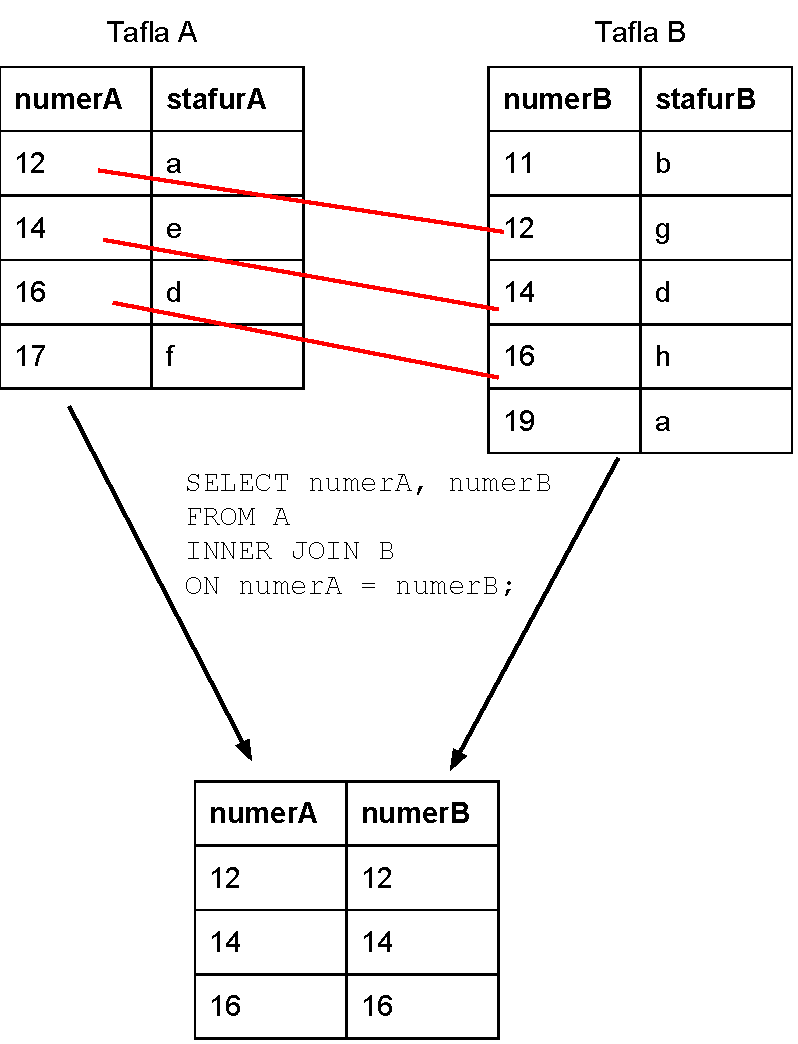
\includegraphics[width=\linewidth]{myndir/inner-join}
\end{figure}

Þar má sjá gildi í tveimur töflum borin saman. Þessi samanburður á sér stað í \verb|ON| hluta skipunarinnar. Hann er líkur samanburði í \verb|WHERE| klausu, en hefur það sérstaka hlutverk að bera saman línur í tveimur mismunandi töflum.

Fyrir utan það að \verb|FROM| klausan er stærri, þá virkar \verb|SELECT| skipun sem velur úr fleiri en einni töflu alveg eins og \verb|SELECT| skipun sem vinnur bara með eina töflu. Hægt er að velja hvaða dálk úr töflunum tveimur sem er.

Sjá má raunverulegri notkun á \verb|INNER JOIN| á sýnidæmi \ref{sql:k6d3-inner-join}.

\begin{example}
\caption[INNER JOIN]{\emph{SELECT} skipun sem velur úr töflunum \emph{Fog} og \emph{Afangar}. Niðurstöðurnar má sjá á mynd \ref{mynd:nidurstada-join}.}
\label{sql:k6d3-inner-join}
\centering
\sql{sql/k6d3-inner-join.sql}
\end{example}

\begin{figure}
\caption[INNER JOIN niðurstaða]{Niðurstaða \emph{SELECT} skipunarinnar í dæmi \ref{sql:k6d3-inner-join}. }
\label{mynd:nidurstada-join}
\centering
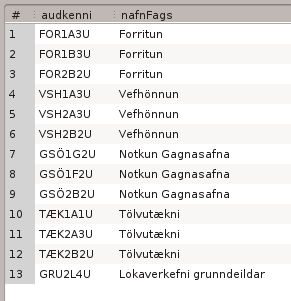
\includegraphics{myndir/workbench-nidurstada-join}
\end{figure}

Hægt er að tengja saman meira en tvær töflur með því að skrifa mörg \verb|JOIN|. Sjá sýnidæmi \ref{sql:k6d4-tvofalt-join}.

\begin{example}
\caption[INNER JOIN]{\emph{SELECT} skipun sem velur nöfn hópa, hvaða áföngum hóparnir tilheyra og hver kennir þá, úr töflunum \emph{Hopar}, \emph{Afangar} og \emph{Starfsmenn}.}
\label{sql:k6d4-tvofalt-join}
\centering
\sql{sql/k6d4-tvofalt-join.sql}
\end{example}

\subsection{OUTER JOIN}
\section{Undirfyrirspurnir}
\label{undirkafli:undirfyrirspurnir}







\chapter{Að uppfæra gagnagrunna}
\label{kafli:uppfaera}
Fyrr í bókinni höfum við farið yfir fjórar grunnaðgerðir sem nauðsynlegar eru til gagnagrunnsvinnslu. Við kunnum að
\begin{itemize}
 \item Búa til gagnagrunna og töflur (\verb|CREATE| skipanir, kaflar \ref{undirkafli:synidaemi-i-sql} og \ref{undirkafli:bua-til-toflu})
 \item Setja gögn inn í töflur (\verb|INSERT| skipunin, \ref{undirkafli:innsetning})
 \item Ná í gögn úr töflum (\verb|SELECT| skipunin, kaflar \ref{kafli:select} og \ref{kafli:gagnavinnslamargartoflur} eins og þeir leggja sig)
 \item Eyða töflum og öllu sem í þeim er (\verb|DROP| skipunin, kafli \ref{undirkafli:drop})
\end{itemize}
Þetta kemur okkur býsna langt. Þetta hefur hins vegar ekki gert okkur kleift að gera nokkrar breytingar á töflum eða þeim gögnum sem í þeim eru. Til þess þurfum við fleiri skipanir. Þær heita \verb|ALTER TABLE|, \verb|UPDATE| og \verb|DELETE|.
\section{DDL og DML}
\begin{marginfigure}[-6cm]
\caption[DDL og DML]{Yfirlit yfir þær SQL-skipanir sem við höfum séð og flokkun þeirra í DDL og DML.}
\label{mynd:ddl-dml}
\centering
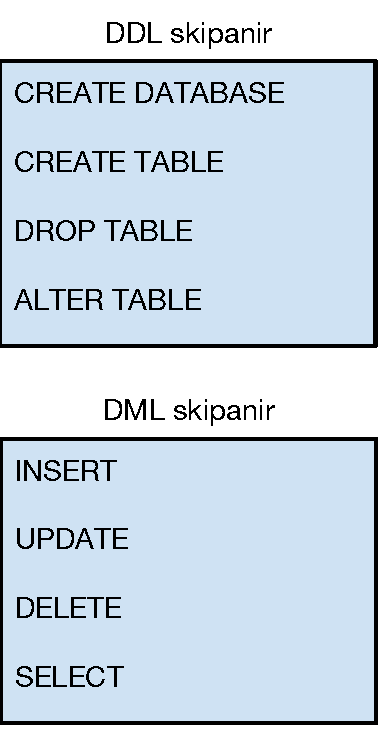
\includegraphics[width=\linewidth]{myndir/ddl-dml}
\end{marginfigure}
Áður en lengra er haldið skulum við staldra við og skoða þær skipanir sem við höfum þegar kynnst.

Þessar skipanir, \verb|CREATE|, \verb|INSERT|, \verb|SELECT| og \verb|DROP| skiptast í tvo flokka. Flokkarnir kallast \emph{Data Definition Language} (DDL) og \emph{Data Manipulation Language} (DML).\footnote{Þessir flokkar hafa verið kallaðir \emph{gagnaskilgreiningarmál} og \emph{gagnameðferðarmál} á íslensku.}

DDL skipanir hafa áhrif á uppbyggingu gagnagrunnsins. Þær breyta, búa til og eyða gagnagrunnum, töflum og dálkum. \verb|CREATE| skipanir og \verb|DROP| skipunin eru DDL skipanir.

DML skipanir hafa áhrif á gögn í gagnagrunninum. Þær breyta, búa til, eyða og sýna innihald taflna. \verb|INSERT| og \verb|SELECT| eru DML skipanir.\footnote{\emph{SELECT} skipunin er örlítið sérstök hvað DML skipanir varðar, þar sem hún hefur það ekki að aðalhlutverki að breyta gögnum. Þess vegna er oft fjallað um hana sérstaklega. Hún er DML skipun engu að síður.}

Fleiri flokkar skipana eru til. Þær skipanir sem við förum yfir í þessari bók falla þó allar í þessa tvo.
\section{Að breyta töflum}
Hingað til höfum við ekki farið yfir leið til að breyta töflum. Það þýðir að í hvert skipti sem villa er gerð í töflu höfum við þurft að henda töflunni ásamt öllu því sem í henni er (\verb|DROP TABLE|) og búa hana til upp á nýtt.

Þetta ferli gengur ekki mjög vel þegar um flókna gagnagrunna eða töflur með raunverulegum gögnum er að ræða. Við þurfum öflugra tól - við þurfum að geta breytt töflu eftir að hún hefur verið búin til.

Til þess að breyta töflu notum við skipunina \verb|ALTER TABLE|. Við getum m.a. notað hana til þess að bæta við og eyða dálkum. Sjá sýnidæmi \ref{sql:k7d1-alter-table}.

\begin{example}
\caption[ALTER TABLE]{Tvær \emph{ALTER TABLE} skipanir. Sú fyrri bætir heiltöludálkinum \emph{nyrDalkur} við töfluna \emph{Tafla}. Sú seinni eyðir dálkinum \emph{gamallaDalkur} úr sömu töflu.}
\label{sql:k7d1-alter-table}
\centering
\sql{sql/k7d1-alter-table.sql}
\end{example}

\verb|ALTER TABLE| breytir einingunum sem í gagnagrunninum eru, töflunum sjálfum. Þess vegna er \verb|ALTER TABLE| DDL-skipun.
\section{Að breyta gögnum}
Fyrir getur komið að við þurfum að breyta töflum. Mun algengari en breytingar á töflum eru þó breytingar á \emph{gögnum}.

Til að breyta gögnum má nota skipunina \verb|UPDATE|. Hún setur ekki inn gögn sjálf (til þess notum við áfram \verb|INSERT| skipanir), hún breytir einungis gögnum sem þegar eru til staðar í gagnagrunninum.

\verb|UPDATE| skipun skiptist í þrjá aðalhluta\footnote{Einnig er hægt að setja \emph{ORDER BY} og \emph{LIMIT} klausur í \emph{UPDATE} skipanir. \emph{ORDER BY} segir til um í hvaða röð \emph{UPDATE} skipunin á að vinna, \emph{LIMIT} setur takmark á það hversu mörgum línum skipunin má breyta.}:
\begin{enumerate}
 \item \verb|UPDATE| lykilorðið og nafnið á töflu eða töflum, sem segir til um hvar gögnin er að finna.
 \item \verb|SET| klausa, sem telur upp þá dálka sem breyta á og nýju gildin sem eiga að fara í þá.
 \item \verb|WHERE| klausa, sem setur skilyrði á þau gögn sem eiga að uppfærast. Eigi engin skilyrði að gilda um gögnin (sem sagt, ef uppfæra á allar viðeigandi línur) má sleppa \verb|WHERE| klausnni. 
\end{enumerate}
Notkun \verb|UPDATE| skipunarinnar má sjá á sýnidæmum \ref{sql:k7d2-update-where} og \ref{sql:k7d3-update}.

\begin{example}
\caption[UPDATE með WHERE]{\emph{UPDATE} skipun sem breytir nemendatöflunni. Hún skráir umsjónarkennara á nemanda númer 4. Umsjónarkennaranúmerið verður 11 eftir að skipunin hefur verið keyrð, óháð fyrra gildi.}
\label{sql:k7d2-update-where}
\centering
\sql{sql/k7d2-update-where.sql}
\end{example}

\begin{example}
\caption[UPDATE án WHERE][1cm]{\emph{UPDATE} skipun sem breytir \emph{allri} nemendatöflunni með því að sleppa \emph{WHERE} klausunni. Þessi skipun myndi skrá alla nemendur í umsjón hjá starfsmanni númer $1$, Bjargeyju.}
\vspace{1cm}
\label{sql:k7d3-update}
\centering
\sql{sql/k7d3-update.sql}
\end{example}

Gætum þess að rugla ekki saman \verb|ALTER| og \verb|UPDATE|. \verb|UPDATE| breytir einungis gögnum, ekki töflum eða öðrum gagnagrunnshlutum. Hún er DML skipun.
\section{Að eyða gögnum}
Þegar eyða þarf gögnum án þess að hafa áhrif á töfluna eða töflurnar sem gögnin eru í má nota \verb|DELETE| skipun. Henni svipar til \verb|UPDATE| skipunarinnar, nema hvað engin \verb|SET| klausa er til staðar - enda eru gögnin fjarlægð, ekki uppfærð.

\begin{example}
\caption[DELETE]{\emph{DELETE} skipun sem eyðir áfanganum \emph{GSÖ1G2U} úr áfangatöflunni. Notuð er \emph{WHERE} klausa til að einangra áfangann líkt og í \emph{UPDATE} skipuninni.}
\label{sql:k7d4-delete}
\centering
\sql{sql/k7d4-delete.sql}
\end{example}

Sé \verb|WHERE| klausunni sleppt í \verb|DELETE| skipun er \emph{öllum} línum eytt. Pössum vandlega upp á að sú klausa sé til staðar og að hún sé rétt!

Líkt og \verb|UPDATE| hefur \verb|DELETE| einungis áhrif á gögn, ekki töflur eða gagnagrunna. Hún er DML skipun.
\section{Viðhald gagnagrunna}
Þegar gagnagrunnum og gögnum í þeim er breytt geta komið upp óvæntar aðstæður. Viðhald gagnagrunna er efni í bók út af fyrir sig, en við getum nefnt nokkur atriði stuttlega.
\subsection{Aðkomulyklar og breytingar}
MySQL passar oftast upp á\footnote{Þetta er stillingaratriði sem hægt er að slökkva á.} að ekki sé hægt að breyta eða eyða gögnum sem aðkomulykill vísar á (gögn sem eru í ``foreldrahlutverki'' í aðkomulykilssambandi) svo að sambandið skemmist.

Einfaldasta leiðin til að komast fram hjá þessu er að breyta eða eyða gögnunum í barninu á undan gögnunum í foreldrinu, svo að það ``loforð'' sem aðkomulykillinn gefur sé aldrei brotið.

Hægt er að setja upp aðkomulykla svo að slíkar breytingar séu sjálfvirkar. Þetta eru svokallaðar \verb|CASCADE| aðgerðir.
\subsection{Hreyfingar} %Transactions
Þegar margar uppfærslur eða breytingar eru framkvæmdar í röð geta komið upp villur ef ferlið er truflað áður en því er lokið.

Til að tryggja það að breytingar sem eru háðar hver annarri séu framkvæmdar sem ein heild má skilgreina þær sem eina \emph{hreyfingu}\footnote{e. \emph{transaction}}. Líkja má SQL-hreyfingu við það þegar fjallgöngukappar binda sig saman í blindbyl; týnist þeir eru þeir þó í það minnsta saman. Hreyfingar eru mikilvægar til að tryggja það að gögn í gagnagrunnum skemmist ekki þegar villur koma upp við breytingar.

\newpage
\section{Yfirlit}
Í þessum kafla fórum við yfir nokkur atriði sem tengjast því að uppfæra gagnagrunna og hinar mismunandi skipanir sem því tengjast.
\begin{itemize}
 \item SQL-skipanir sem við höfum farið yfir skiptast í tvo flokka, DDL og DML.
 \item DDL skipanir búa til, breyta og eyða gagnagrunnum og töflum.
 \begin{itemize}
  \item \verb|CREATE DATABASE|, \verb|CREATE TABLE|, \verb|ALTER TABLE| og \verb|DROP TABLE| eru DDL-skipanir.
 \end{itemize}
 \item DML-skipanir sýna, setja inn, breyta eða eyða \emph{gögnum} í gagnagrunnum án þess að hafa áhrif á gagnagrunninn sjálfan.
 \begin{itemize}
  \item \verb|SELECT|, \verb|INSERT|, \verb|UPDATE| og \verb|DELETE| eru DML-skipanir.
 \end{itemize}
 \item \verb|ALTER TABLE| skipunin bætir við og eyðir dálkum taflna.
 \item \verb|UPDATE| skipunin breytir gögnum sem eru í töflum.
 \item \verb|DELETE| skipunin eyðir gögnum sem eru í töflum.
\end{itemize}


\chapter{Ítarefni}
\label{kafli:itarefni}
\section{Views}
\label{undirkafli:views}
Sú leið sem notuð er til að geyma gögn í gagnagrunnum er ekki alltaf sú leið sem hentar best til að vinna með gögnin.

Við getum til dæmis skoðað Tækniskólagagnagrunninn sem við bjuggum til í kafla \ref{kafli:uppsetninggagnagrunns} (sjá mynd \ref{mynd:eer}). Sá gagnagrunnur inniheldur þó nokkuð margar töflur, oft þarf að nota \verb|JOIN| (sjá undirkafla \ref{undirkafli:join}) á töflurnar sem í honum eru til að fá upplýsingarnar sem óskað er eftir. T.d. þarf að fara í gegnum þrjár töflur til að finna hvaða kennari kennir hvaða áfanga í Tækniskólagagnagrunninnum (sjá sýnidæmi \ref{sql:k6d4-tvofalt-join}).

Það að þurfa sífellt að framkvæma svipaðar, en flóknar fyrirspurnir til að ná í gögn getur verið afskaplega þreytandi. Einfaldara væri ef við værum alltaf með akkúrat þær upplýsingar sem við þurfum, á því sniði sem við þurfum.

\begin{figure}
\caption[View]{Gagnagrunnur með ``Views''}
\label{mynd:view}
\centering
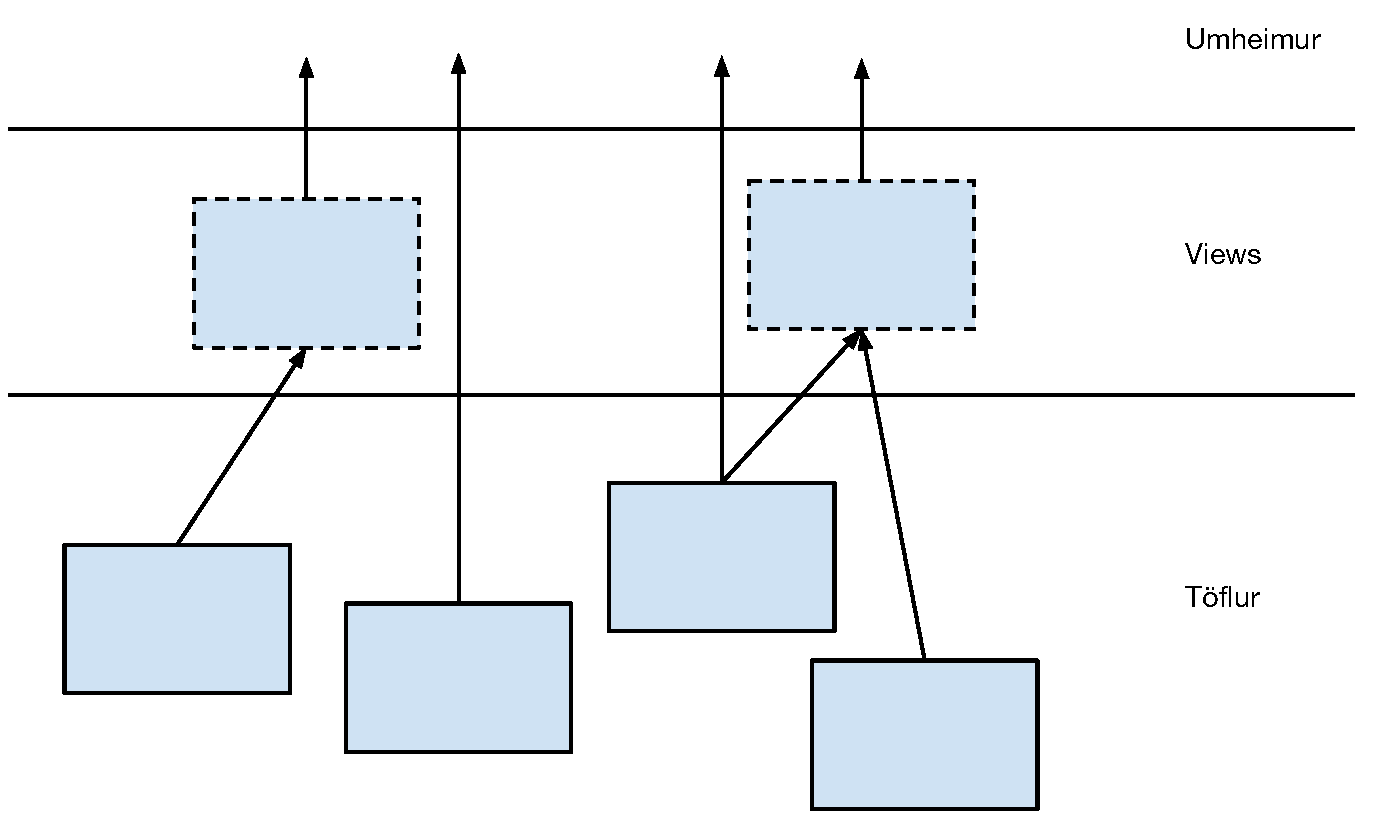
\includegraphics[width=\linewidth]{myndir/views}
\end{figure}

Til að auðvelda líf okkar í þessum aðstæðum getum við búið til svokölluð \emph{View}. View er nokkurs konar ``sýndartafla'' sem skilgreint er af niðurstöðum fyrirspurnar.

Til að búa til View notum við DDL-skipunina\footnote{sjá DDL og DML í kafla \ref{kafli:uppfaera}} \verb|CREATE VIEW|. Einföld \verb|CREATE VIEW| skipun er byggð upp á eftirfarandi hátt: Fyrst kemur nafn skipunarinnar (\verb|CREATE VIEW|), svo nafnið sem við ætlum að gefa view-inu, svo lykilorðið \verb|AS| og að lokum fyrirspurnin (\verb|SELECT|) sem view-ið á að byggjast á. Sjá sýnidæmi \ref{sql:k8d1-create-view}

\begin{example}
\caption[View]{\emph{CREATE VIEW} skipun. Þessi skipun býr til sýndartöflu sem einfaldar aðgang að upplýsingum um hvaða kennari kennir hvaða áfanga.}
\label{sql:k8d1-create-view}
\centering
\sql{sql/k8d1-create-view.sql}
\end{example}

Þegar view-ið hefur verið búið til má senda á það fyrirspurnir eins og hverja aðra töflu í gagnagrunninum. Sjá sýnidæmi \ref{sql:k8d2-select-from-view}.

\begin{example}
\caption[SELECT úr view]{Kennarar sem kenna \emph{FOR1A3U} fundnir með því að senda fyrirspurn á view-ið sem búið var til í sýnidæmi \ref{sql:k8d1-create-view}. }
\label{sql:k8d2-select-from-view}
\centering
\sql{sql/k8d2-select-from-view.sql}
\end{example}

View hafa nokkra kosti aðra en að minnka flækjustig algengra aðgerða. T.d. er hægt að nota view til að koma (e.t.v. tímabundið) í stað töflu sem hefur verið breytt, svo niðurstöður fyrirspurna sem hafa verið skrifaðar breytist ekki þó að gagnagrunnurinn hafi verið uppfærður. Einnig er hægt að nota view til að stýra aðgangi að gagnagrunnum. T.d. er hægt að gefa notanda gagnagrunns aðgang að töflu sem inniheldur trúnaðarupplýsingar án þess að notandinn komist í þær upplýsingar með því að búa til view á töfluna sem inniheldur þær upplýsingar sem notandinn þarf, og gefa notandanum svo aðgang að view-inu en fela töfluna.
\section{Yfirlit yfir helstu gagnagrunnskerfi}
\label{undirkafli:helstu-gagnagrunnskerfi}
Gríðarmörg SQL-gagnagrunnskerfi eru til. Í þessum undirkafla verða þau gagnagrunnskerfi sem höfundur telur líklegast að nemendur Tækniskólans muni rekast á í náinni framtíð kynnt.

Grundvallaratriði SQL, sem farið er yfir í þessari bók, hafa miðast við notkun MySQL (\ref{undirkafli:mysql}). Hugmyndirnar á bak við þessi grundvallaratriði er sú sama í öllum gagnagrunnskerfum sem byggja á SQL, en \emph{útfærslan} er ekki endilega sú sama. Við skulum ekki búast við því að sýnidæmi bókarinnar keyri óbreytt í öllum gagnagrunnskerfum.
\subsection{MySQL}
\label{undirkafli:mysql}
\begin{marginfigure}
\caption{MySQL}
\label{mynd:mysql}
\centering

\includegraphics[width=\linewidth]{myndir/mysql}
\end{marginfigure}
MySQL\footnote{\url{http://www.mysql.com/}} er gagnagrunnskerfi í mikilli notkun, sérstaklega við vefsíðugerð.

Þökk sé útbreiðslunni er tiltölulega auðvelt að finna leiðbeiningar um notkun MySQL og uppsetningu MySQL-servera. Hægt er að vinna með MySQL í gegnum fjölmörg forritunarmál. MySQL er opið\footnote{e. \emph{open source}} og ókeypis.

MySQL hefur skilist að í nokkra hluta síðan það var fyrst gefið út. Upprunalegir höfundar kerfisins vinna nú við afbrigði sem heitir MariaDB\footnote{\url{https://mariadb.org/}}.
\subsection{PostgreSQL}
\begin{marginfigure}
\caption{PostgreSQL}
\label{mynd:postgresql}
\centering

\includegraphics[width=0.8\linewidth]{myndir/postgresql}
\end{marginfigure}
PostgreSQL\footnote{\url{http://www.postgresql.org/}} er gagnagrunnskerfi sem leggur mikla áherslu á að fylgja stöðlum og bjóða upp á ``rétta'' gagnavinnslu.

PostgreSQL er vinsælt meðal gagnagrunnssérfræðinga, m.a. vegna þess hversu mikla stjórn gagnagrunnstjórinn hefur yfir virkni kerfisins. Kennt er á PostgreSQL gagnasafnsfræðiáföngum Tækniskólans.

Fyrir utan það að styðja ``venjulegar'' SQL skipanir, þá býður PostgreSQL upp á forritunarmál, kallað PL/pgSQL (Procedural Language/PostgreSQL), til að auðvelda ýmsar aðgerðir. PL/pgSQL býður meðal annars upp á lykkjur og önnur tól sem kunnugleg eru úr forritunarmálum á borð við C\#.
\subsection{SQLite}
\begin{marginfigure}
\caption{SQLite}
\label{mynd:sqlite}
\centering

\includegraphics[width=\linewidth]{myndir/sqlite}
\end{marginfigure}
SQLite\footnote{\url{http://sqlite.org/}} er ólíkt flestum gagnagrunnskerfum að því leyti að ekki þarf að setja upp eiginlegt kerfi á tölvunni sem á að hýsa gagnagrunninn, allt forritið er ein skrá.

Smæðarinnar vegna vantar SQLite ýmsa eiginleika sem stærri gagnagrunnskerfi bjóða upp á, en það hentar sérstaklega vel til að nota sem hluta af stærri kerfum. SQLite má finna ``undir húddinu'' á mörgum forritum sem þurfa að geyma gögn.
\subsection{Microsoft SQL Server}
\begin{marginfigure}
\caption{SQL Server}
\label{mynd:sql-server}
\centering

\includegraphics[width=\linewidth]{myndir/sql-server}
\end{marginfigure}
SQL Server\footnote{\url{http://www.microsoft.com/sqlserver}} er gagnagrunnskerfi gefið út af Microsoft. Það er sniðið til að passa vel til keyrslu á Windows-vélum. SQL Server er helsti keppinautur Oracle gagnagrunnskerfisins þegar kemur að stórum gagnagrunnum.

Sú útgáfa af SQL sem notuð er til samskipta við SQL Server heitir Transact-SQL. T-SQL styður lykkjur og breytur.
\subsection{Oracle Database}
\label{undirkafli:oracle}
\begin{marginfigure}
\caption{Oracle Database}
\label{mynd:oracle}
\centering

\includegraphics[width=\linewidth]{myndir/oracle}
\end{marginfigure}
Gagnagrunnskerfi Oracle\footnote{\url{http://www.oracle.com/us/products/database/overview/}} er mest notaða gagnagrunnskerfi í heimi í dag. Það hefur verið í þróun áratugum saman og knýr marga af heimsins stærstu gagnagrunnum.

Útvíkkun Oracle á SQL til að styðja lykkjur og önnur algeng forritunaratriði er kallað PL/SQL (Procedural Language/Structured Query Language).
\section{Venslalíkanið}
SQL byggir á föstum stærðfræðilegum grunni. Sá grunnur er kallaður \emph{venslalíkanið}\footnote{e. \emph{Relational model}}. Því var fyrst lýst af tölvunarfræðingnum Edgar Codd um 1970\footnote{Aðalgreinin sem lýsir því heitir ``\emph{A Relational Model of Data for Large Shared Data Banks}''. Áhugasamir geta fundið hana á netinu.}.

Venslalíkanið lýsir því hvernig líta má á gögn sem stök í mengjum og hvernig nota má þekktar\footnote{Þær eru í það minnsta þekktar flestum stærðfræðingum.} stærðfræðiaðgerðir til að nálgast þær. 

SQL er \emph{útfærsla} á venslalíkaninu. Uppbygging þess leiðir til þess að þegar við tölum um SQL notum við sjaldnast sama orðaforða og er notaður í stærðfræðinni sem það byggir á. Engu að síður er skilningur á venslalíkaninu og þeim orðaforða sem þar kemur við sögu mjög gagnlegur öllum sem nota SQL.

Ítarleg umfjöllun um venslalíkanið er viðfangsefni fyrir háskólanámskeið, ekki þessa bók. Engu að síður skulum við skoða mikilvægasta hugtak líkansins, \emph{vensl}, og hvernig það passar við það sem við höfum séð af SQL í þessari bók.
\subsection{Mengi}
Áður en lengra er haldið skulum við vera viss um að við höfum hugmynd um hvað \emph{mengi}\footnote{e. \emph{set}} er. Þetta eru sömu mengin og við höfum kynnst í grunnskólastærðfræði.

Mengi er safn/hópur af fyrirbærum. ``Fyrirbærin'' í mengi geta verið nær hvað sem er, t.d. tölur, orð, eða önnur mengi. ``Heiltölur'', ``Íslendingar'' og ``Rauðir hlutir'' eru allt mengi.

Tvö atriði einkenna mengi:
\begin{itemize}
 \item Röð hluta í mengi skiptir ekki máli.
 \item Aldrei er um endurtekningar að ræða í mengi. Hlutur er annaðhvort í mengi eða hann er það ekki.
\end{itemize}
Þegar hlutur er í mengi er talað um að hluturinn sé \emph{stak} í menginu.

Mengjum er oft gefið nafn sem er einn stór bókstafur. T.d. er algengt að kalla mengi heiltalna $N$. 

Þetta gerir okkur mögulegt að kynnast fleiri hugtökum. Skoðum tvö mengi, $A$ og $B$. Það skiptir okkur ekki máli hvað er í mengjunum.
\begin{itemize}
 \item Séu öll stök í mengi $A$ líka stök í mengi $B$ er sagt að $A$ sé \emph{hlutmengi} $B$.
 \item Séu einhver stök í mengi $A$ sem líka eru í mengi $B$ er sagt að þau stök séu í \emph{sniðmengi} $A$ og $B$.
 \item Mengi sem inniheldur öll stök úr mengjum $A$ og $B$ er kallað \emph{sammengi} $A$ og $B$.
\end{itemize}


\subsection{Vensl}
Við skulum sjá fyrir okkur mörg mengi af upplýsingum. Köllum þau öll $S$ og gefum þeim númer, svo við getum kallað þau $S_1, S_2$ og svo framvegis.

Skoðum nú annað mengi og köllum það $R$. Mengið $R$ er \emph{vensl\footnote{e. \emph{relation}} á mengin $S$} ef $R$ er mengi af \emph{línum}\footnote{e. \emph{tuples}} þar sem að fyrsta gildið í línunni er úr $S_1$, annað stakið úr $S_2$, og svo framvegis.

Til að gera venslin nothæf getum við ákveðið að hvert mengi $S$ standi fyrir einhvern ákveðinn \emph{eiginleika}\footnote{e. \emph{attribute}} sem gögn geta haft. Þá stendur hver lína í venslunum fyrir einn ``hlut'' sem einkennist af þeim eiginleikum sem við skilgreindum.

Hvernig tengist þetta þeim hugtökum sem við höfum lært úr SQL?

\begin{itemize}
 \item Lína í SQL-töflu samsvarar (e. \emph{tuple}) í venslum.
 \item Dálkur í SQL-töflu samsvarar eiginleika (e. \emph{attribute}) í venslum.
 \item SQL-tafla samsvarar að mestu leyti venslum.\footnote{Vensl og SQL-töflur greinast að á nokkrum atriðum. T.d. eru vensl alvöru mengi, sem ekki geta verið með endurtekningar. SQL-tafla sem ekki er með aðallykil getur innihaldið endurtekin gildi.}
 \item Niðurstöður fyrirspurna og view-a (sjá undirkafla \ref{undirkafli:views}) samsvara líka að mestu leiti venslum.
\end{itemize}

Það að skilja venslalíkanið gerir sum atriði sem viðkoma SQL skýrari, t.d. samband view-a og taflna. Einnig getum við nú séð að þegar rætt er um venslaðar töflur er átt við töflur sem hægt er að búa til vensl á.


\section{Að tengjast gagnagrunni með PHP}
\label{undirkafli:php}
Við höfum eytt miklum tíma í að skoða gagnagrunna sem sjálfstætt fyrirbrigði.

Í þessum undirkafla skoðum við loksins hvernig tengja má MySQL-gagnagrunn við PHP-forritskóða.
Slíkar tengingar eru teknar fyrir vegna þess hve algengar\footnote{Linux, Apache, PHP og MySQL mynda saman ``pakka'' sem oft er notaður sem ein heild. Pakkinn er nefndur eftir skammstöfun sinni, LAMP. Hann er í gríðarmikilli notkun.} þær eru í vefforritun.

Útskýringarnar gera ráð fyrir skilningi á ýmsum atriðum:
\begin{itemize}
 \item Hugtökum í vefsíðum - HTML, Javascript
 \item Keyrslu PHP-skripta
 \item Grundvallarmálfræði PHP
 \item IP-tölum
 \item Föllum, lykkjum og fylkjum\footnote{e. \emph{functions}, \emph{loops} og \emph{arrays}}
\end{itemize}
\subsection{Hlutverk gagnagrunna í vefsíðum}
Vefsíða sem byggð er upp á hefðbundinn hátt skiptist gróflega í tvo hluta - client og server. 

\begin{figure}
\centering
\caption{Hefðbundin uppbygging vefsíðu}
\label{mynd:uppbyggingvefsidu}
\color{red} Hingað kemur falleg mynd af client-server strúktúr vefsíðu.
\end{figure}

Client-hlutinn er sá hluti sem keyrður er á tölvu notandans. Í client-hluta eru HTML-tög túlkuð og Javascript-kóði keyrður, m.a.. Venjulega fer þessi vinna fram í vafra\footnote{e. \emph{browser}, t.d. Google Chrome, Firefox og Internet Explorer} notandans.

Server-hlutinn er margskiptur. Viðfangsefni okkar, PHP og MySQL, tilheyra þessum hluta. Oft keyra PHP og MySQL á sömu tölvu, sem er þá einfaldlega nefnd ``serverinn''.

Hlutverk gagnagrunnsins í þessari uppbyggingu er, eðli hans samkvæmt, það að halda utan um upplýsingar. PHP-hluti serversins sér um að eiga samskipti við gagnagrunninn og miðla upplýsingunum áfram til clientsins. Notandinn og tölva hans eiga aldrei bein samskipti við MySQL-serverinn.

\subsection{Uppsetning tengingar með PDO}
Gerum ráð fyrir að við séum með PHP-skriptu sem keyrir á vefþjóni. Til að tengjast MySQL-gagnagrunni þarf hún eftirfarandi upplýsingar:
\begin{itemize}
 \item Tengingarupplýsingar: Gagnagrunnsgerðina (hjá okkur alltaf MySQL), nafn gagnagrunnsins og staðsetningu hans
 \item Notandanafn MySQL-þjónsins
 \item Lykilorð notandans.
\end{itemize}
Klasann \href{http://www.php.net/manual/en/class.pdo.php}{PDO}\footnote{\url{http://www.php.net/manual/en/class.pdo.php}} má svo nota til þess að mynda tenginguna sjálfa.\footnote{Fleiri leiðir eru færar til að mynda tengingar af þessum toga, til dæmis \emph{mysqli} viðbótin. Þá PHP-viðbót sem einfaldlega heitir \emph{mysql} skal þó alls ekki nota - hún er úreld.}

\begin{example}[h]
\caption{Tenging við gagnagrunn með PDO}
\label{sql:k8d1}
\centering
\inputminted[frame=lines, fontfamily=courier]{php}{php/k8d1.php}
\end{example}

Dæmi um hvernig öll skriptan gæti litið út má sjá á sýnidæmi \ref{sql:k8d1}. Skoðum það sýnidæmi nánar. 

Fyrsta breytan sem er skilgreind í skriptunni (\verb|$source|) inniheldur tengingarupplýsingarnar. Þar kemur fyrst fram orðið \verb|mysql|, aðskilið frá gagnagrunnsnafninu og staðsetningu gagnagrunnins með tvípunkti. Sé ætlunin að skrifa skriptu af þessum toga til nota í eigin forriti þyrfti að skipta út \verb|testdb| fyrir nafn gagnagrunnsins sem nota skal. Sé MySQL-serverinn ekki að keyra á sömu tölvu og PHP-skriptan þarf einnig að breyta IP-tölunni í IP-tölu tölvunnar sem MySQL-serverinn keyrir á.

Næstu tvær breytur innihalda notandanafn og lykilorð fyrir MySQL-serverinn. Þetta er sama notandanafn og lykilorð og notað var til að tengjast gagnagrunninum í kafla \ref{kafli:fyrstuskrefin}.

Þegar upplýsingarnar hafa verið geymdar er loks ``reynt'' að búa til tengingu með PDO. Takist það eru tengingarupplýsingarnar geymdar í  ``database handle'' breytu, nefnd \verb|$dbh| í sýnidæminu. Þessa breytu má síðan nýta til að eiga samskipti við gagnagrunninn.

Takist ekki að koma tengingunni á prentar skriptan út strenginn ``Tenging mistókst'' ásamt villuskilaboðunum sem berast.
\subsection{Að sækja gögn með PDO}
\subsection{Að birta gögn á vefsíðu}
\end{document}